\documentclass[usenames,dvipsnames,mathserif,notheorems]{beamer}

% silence annoying warnings
\usepackage{silence}
\usepackage{caption}
\WarningFilter{remreset}{The remreset package}
\usepackage{xcolor}
\usepackage{algorithm}
\usepackage{algorithmic}
\usepackage{centernot}
\usepackage{algorithmic}
\usepackage{ulem}

%% Math macros for LaTex Projects 
%% Maintainer: Aaron Mishkin <amishkin@cs.stanford.edu>
%% Original Source: Mark Schmidt (UBC CS), Ben Bloem-Reddy (UBC Stats).

%% Easy bold-face 

\def\bfA{\mathbf{A}}
\def\bfB{\mathbf{B}}
\def\bfC{\mathbf{C}}
\def\bfD{\mathbf{D}}
\def\bfE{\mathbf{E}}
\def\bfF{\mathbf{F}}
\def\bfG{\mathbf{G}}
\def\bfH{\mathbf{H}}
\def\bfI{\mathbf{I}}
\def\bfJ{\mathbf{J}}
\def\bfK{\mathbf{K}}
\def\bfL{\mathbf{L}}
\def\bfM{\mathbf{M}}
\def\bfN{\mathbf{N}}
\def\bfO{\mathbf{O}}
\def\bfP{\mathbf{P}}
\def\bfQ{\mathbf{Q}}
\def\bfR{\mathbf{R}}
\def\bfS{\mathbf{S}}
\def\bfT{\mathbf{T}}
\def\bfU{\mathbf{U}}
\def\bfV{\mathbf{V}}
\def\bfW{\mathbf{W}}
\def\bfX{\mathbf{X}}
\def\bfY{\mathbf{Y}}
\def\bfZ{\mathbf{Z}}

% bb series
\def\bbA{\mathbb{A}}
\def\bbB{\mathbb{B}}
\def\bbC{\mathbb{C}}
\def\bbD{\mathbb{D}}
\def\bbE{\mathbb{E}}
\def\bbF{\mathbb{F}}
\def\bbG{\mathbb{G}}
\def\bbH{\mathbb{H}}
\def\bbI{\mathbb{I}}
\def\bbJ{\mathbb{J}}
\def\bbK{\mathbb{K}}
\def\bbL{\mathbb{L}}
\def\bbM{\mathbb{M}}
\def\bbN{\mathbb{N}}
\def\bbO{\mathbb{O}}
\def\bbP{\mathbb{P}}
\def\bbQ{\mathbb{Q}}
\def\bbR{\mathbb{R}}
\def\bbS{\mathbb{S}}
\def\bbT{\mathbb{T}}
\def\bbU{\mathbb{U}}
\def\bbV{\mathbb{V}}
\def\bbW{\mathbb{W}}
\def\bbX{\mathbb{X}}
\def\bbY{\mathbb{Y}}
\def\bbZ{\mathbb{Z}}

% cal series
\def\calA{\mathcal{A}}
\def\calB{\mathcal{B}}
\def\calC{\mathcal{C}}
\def\calD{\mathcal{D}}
\def\calE{\mathcal{E}}
\def\calF{\mathcal{F}}
\def\calG{\mathcal{G}}
\def\calH{\mathcal{H}}
\def\calI{\mathcal{I}}
\def\calJ{\mathcal{J}}
\def\calK{\mathcal{K}}
\def\calL{\mathcal{L}}
\def\calM{\mathcal{M}}
\def\calN{\mathcal{N}}
\def\calO{\mathcal{O}}
\def\calP{\mathcal{P}}
\def\calQ{\mathcal{Q}}
\def\calR{\mathcal{R}}
\def\calS{\mathcal{S}}
\def\calT{\mathcal{T}}
\def\calU{\mathcal{U}}
\def\calV{\mathcal{V}}
\def\calW{\mathcal{W}}
\def\calX{\mathcal{X}}
\def\calY{\mathcal{Y}}
\def\calZ{\mathcal{Z}}


%% Theorem Environments %%
\usepackage{amsthm}
\usepackage{thmtools, thm-restate}
\declaretheorem{theorem}
\declaretheorem{proposition}
\declaretheorem{remark}
\declaretheorem{lemma}
\declaretheorem{definition}
\declaretheorem{assumption}
\declaretheorem{corollary}
\declaretheorem{example}

%% Floor and Ceiling %%
\usepackage{mathtools} % required for \DeclarePairedDelimeter

%% Stochastic Relations %% 

% almost sure:
\newcommand{\as}[1]{\stackrel{\text{\rm\tiny a.s.}}{#1}}
% a.s.\ equality:
\newcommand{\equas}{\stackrel{\text{\rm\tiny a.s.}}{=}}

% in distribution:
\newcommand{\dist}[1]{\stackrel{\text{\rm\tiny dist}}{#1}}
% equality in distribution:
\newcommand{\equdist}{\stackrel{\text{\rm\tiny dist}}{=}}

% independent
\newcommand{\ind}[0]{\perp \!\!\! \perp }

%% Variance, Expectation, etc %%
\newcommand{\Var}[1]{\textbf{Var}\sbr{#1}}

% ceiling and floor
\DeclarePairedDelimiter{\ceil}{\lceil}{\rceil}
\DeclarePairedDelimiter{\floor}{\lfloor}{\rfloor}
\newcommand{\argdot}{{\,\vcenter{\hbox{\tiny$\bullet$}}\,}} %generic argument dot

% absolute value
\newcommand{\abs}[1]{\left\vert #1\right\vert}

\newcommand{\seq}[1]{\rbr{#1}}

% easy bracketing:
\newcommand{\rbr}[1]{\left(#1\right)}
\newcommand{\sbr}[1]{\left[#1\right]}
\newcommand{\cbr}[1]{\left\{#1\right\}}
\newcommand{\abr}[1]{\left\langle#1\right\rangle}

% Norms
\def\norm#1{\|#1\|}
\def\biggnorm#1{\bigg\|#1\bigg\|}
% Random Variable Norms:
\def\psitwo#1{\|#1\|_{\psi_2}}
\def\psione#1{\|#1\|_{\psi_1}}

% mid
\newcommand{\biggmid}{\bigg \vert }

% argmax/argmin
\def\argmax{\mathop{\rm arg\,max}}
\def\argmin{\mathop{\rm arg\,min}}

% General Symbols
\def\half{\frac 1 2}
\newcommand{\inv}[1]{\frac{1}{#1}}
\newcommand{\halved}[1]{\frac{#1}{2}}
\newcommand{\R}{\mathbb{R}}
\newcommand{\eR}{\bar{\mathbb{R}}}

\newcommand{\into}{\rightarrow}

% Gradient Descent Symbols
\newcommand{\oracle}{\mbox{\( \calO \)}}
\newcommand{\iter}{k}

\newcommand{\Lk}{L_{\zk}}
\newcommand{\Lmax}{L_{\text{max}}}
\newcommand{\mumax}{\mu_{\text{max}}}
\newcommand{\Lmin}{L_{\text{min}}}
\newcommand{\mumin}{\mu_{\text{min}}}

% iterates
\newcommand{\y}{y}
\newcommand{\yk}{y_k}
\newcommand{\ykk}{y_{k+1}}

\newcommand{\vk}{v_k}
\newcommand{\vkk}{v_{k+1}}

\newcommand{\w}{w}
\newcommand{\wk}{w_k}
\newcommand{\wkk}{w_{k+1}}
\newcommand{\wopt}{w^*}
\newcommand{\wbar}{\bar{w}}


\newcommand{\x}{x}
\newcommand{\xk}{x_k}
\newcommand{\xkplus}{x_k^+}
\newcommand{\xkk}{x_{k+1}}
\newcommand{\xopt}{x^*}
\newcommand{\xbar}{\xbar{w}}

% noise
\newcommand{\Z}{Z}
\newcommand{\z}{z}
\newcommand{\zk}{z_{k}}
\newcommand{\zkk}{z_{k+1}}
% step-sizes
\newcommand{\tetak}{{\tilde{\eta}}_{k}}
\newcommand{\etamin}{\eta_{\text{min}}}
\newcommand{\etamax}{\eta_{\text{max}}}
\newcommand{\etak}{\eta_k}
\newcommand{\etakk}{\eta_{k+1}}

\newcommand{\betak}{\beta_{k}}
\newcommand{\betakk}{\beta_{k+1}}
\newcommand{\alphak}{\alpha_{k}}
\newcommand{\alphakk}{\alpha_{k+1}}

\newcommand{\Ek}{\bbE_{\zk}}
\newcommand{\E}{\bbE}

% functions
\newcommand{\f}{f}
\newcommand{\fj}{f_i}
\newcommand{\fopt}{f^*}
% sub-sampled functions
\newcommand{\fk}{f_{i_k}}
\newcommand{\fkk}{f_{i_{(k+1)}}}
% gradients
\newcommand{\grad}{\nabla f}
% sub-sampled gradients
\newcommand{\gradk}{\nabla f_{i_k}}
\newcommand{\gradkk}{\nabla f_{i_{(k+1)}}}

%% Weak and strong growth constants
\newcommand{\sgc}{\rho}
\newcommand{\wgc}{\alpha}
%%%%%%%%%%%%%%%%%%%%%%%%%%%%%%%%%%%%%%%%%%%%%%%%%%%%%%%%%%


%% Etc %%  

%% add numbers to align* environments.
\newcommand{\addnumber}{\addtocounter{equation}{1}\tag{\theequation}}

%%%%%%%%%

%% Group Lasso %%
\newcommand{\bi}{{i}}
\newcommand{\wi}{w_\bi}
\newcommand{\vi}{v_\bi}
\newcommand{\ci}{c_\bi}
\newcommand{\zi}{z_\bi}
\newcommand{\Xbi}{X_\bi}
\newcommand{\act}{{\calA_{\lambda}}}
\newcommand{\inact}{{\calI_{\lambda}}}
\newcommand{\tran}{{\calT_{\lambda}}}
\newcommand{\equi}{{\calE_{\lambda}}}

\newcommand{\acts}{{\calA_{\lambda}^{*}}}
\newcommand{\trans}{{\calT_{\lambda}^{*}}}

\newcommand{\wa}{w_\act}
\newcommand{\was}{w_\acts}
\newcommand{\we}{w_\equi}
\newcommand{\va}{v_\act}
\newcommand{\vas}{v_\acts}
\newcommand{\ca}{c_\act}
\newcommand{\cas}{c_\acts}
\newcommand{\ve}{v_\equi}
\newcommand{\ce}{c_\equi}
\newcommand{\Xa}{X_\act}
\newcommand{\Xas}{X_\acts}
\newcommand{\Xe}{X_\equi}

\newcommand{\wmin}{w^*}
\newcommand{\solfn}{\calW^*}

\newcommand{\Null}{\text{Null}}
\newcommand{\Row}{\text{Row}}
\newcommand{\Span}{\text{Span}}
\newcommand{\Range}{\text{Range}}

\newcommand{\Di}{\calD_{\bi}}
\newcommand{\Si}{\calN_{\bi}}
\newcommand{\Dis}{\Di^{*}}
\newcommand{\Sis}{\Ni^{*}}
\newcommand{\Ds}{\calD^{*}_\lambda}
\newcommand{\Ss}{\calN^{*}_\lambda}

\newcommand{\Ki}{K_{\bi}}
\newcommand{\Kid}{K_{\Di}}
\newcommand{\Kids}{K_{\Di^*}}
\newcommand{\Kd}{K_{\calD}}
\newcommand{\Kda}{K_{\calD \cap \act}}
\newcommand{\Kdas}{K_{\Gs}}
\newcommand{\Ka}{K_\act}

\newcommand{\Gs}{\calG^{*}_{\lambda}}

% dual parameters
\newcommand{\ri}{\rho_{\bi}}
\newcommand{\ract}{\rho_{\act}}
\newcommand{\racts}{\rho_{\acts}}
\newcommand{\rid}{\rho_{\Di}}
\newcommand{\rd}{\rho_{\calD}}
\newcommand{\rda}{\rho_{\calD \cap \act}}
\newcommand{\rdas}{\rho_{\Gs}}
\newcommand{\ra}{\rho_{\act}}
\newcommand{\rmin}{\rho^*}

\newcommand{\vmin}{v^*}
\newcommand{\diag}{\text{diag}}
\newcommand{\nnz}{\text{nnz}}

\newcommand{\tmu}{\tilde{\mu}}
\newcommand{\tL}{\tilde{L}}

%% Plotting macros for LaTex Projects 
%% Maintainer: Aaron Mishkin <amishkin@cs.stanford.edu>


%% Tikz and PGFplots packages
\usepackage{tikz}
\usepackage{pgfplots}

% tikz and PGFplots libraries
\usepgfplotslibrary{fillbetween}
\usetikzlibrary{patterns}



%% tikz settings 
\tikzset{
    font={\fontsize{12pt}{12}\selectfont},
}

%% PGFplots settings 
\pgfplotsset{
    % version compatibility
    compat=1.5.1,
    % basic line-styles
    primary/.style={color=black, style=solid, line width=1.5pt}, 
    secondary/.style={color=red, style=solid, line width=1.5pt}, 
}


%% Pause in align environments: https://tex.stackexchange.com/questions/16186
\makeatletter
\let\save@measuring@true\measuring@true
\def\measuring@true{%
	\save@measuring@true
	%\def\beamer@sortzero##1{\beamer@ifnextcharospec{\beamer@sortzeroread{##1}}{}}%
	\def\beamer@sortzeroread##1<##2>{}%
	\def\beamer@finalnospec{}%
}
\makeatother

\pgfdeclarelayer{ft}
\pgfdeclarelayer{bg}
\pgfsetlayers{bg,main,ft}

\pgfplotsset{
	compat=1.5.1,
	oracle/.style={color=red, style=dashed, line width=1.5pt},
	bound/.style={color=blue, style=solid, line width=1.5pt},
	objective/.style={color=black, style=solid, line width=1.5pt},
}

\usepackage{simplebeam}
\usetheme{simplebeamer}

\usetikzlibrary{shapes, arrows}
\usetikzlibrary{decorations.pathreplacing, calligraphy, overlay-beamer-styles}

% node styles
\tikzstyle{Input}=[minimum size=0.3cm, fill=black, line width = 0.5mm, draw=black, shape=circle, text=black]
\tikzstyle{Hidden}=[minimum size=0.3cm, fill=blue, line width = 0.5mm, draw=blue, shape=circle, text=blue]
\tikzstyle{Splits}=[inner sep=0.03cm, minimum size=0.3cm, line width = 0.3mm, draw=blue, shape=circle, text=black]
\tikzstyle{Output}=[minimum size=0.3cm, fill=white, line width = 0.5mm, draw=black, shape=circle, text=black]

% Edge styles
\tikzstyle{arrow}=[line width = 0.5mm]

% bib resources

\addbibresource[]{refs.bib}

\title{Level Set Teleportation: An Optimization Perspective}
\subtitle{\vspace{1ex} AISTATS 2025}
\author{Aaron Mishkin \and Alberto Bietti \and Robert M. Gower}
\collaborators{
    \vspace{-1ex}
	
\includegraphics[width=0.18\linewidth]{assets/flatiron_small.jpeg}
	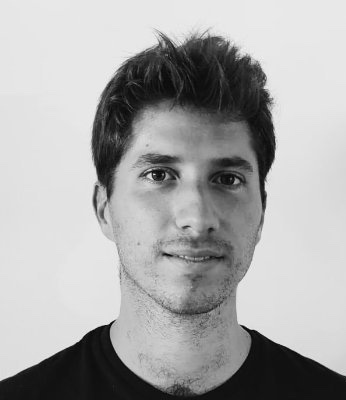
\includegraphics[width=0.18\linewidth]{assets/alberto.jpg}
	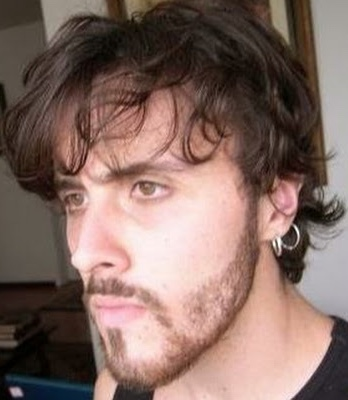
\includegraphics[width=0.18\linewidth]{assets/rob.jpg}
}

\titlegraphic{
\includegraphics[width=0.275\textwidth]{assets/CCM.png}\hfill%

\includegraphics[width=0.4\textwidth]{assets/SUSig_2color_Stree_Left.eps}}

\newcommand{\horizontalrule}{
	{
			\vspace{-0.5em}
			\center \rule{\textwidth}{0.1em}
			\vspace{-0.2em}
		}
}

\definecolor{bad}{HTML}{eb6223}
\definecolor{good}{HTML}{9434ed}

\newcommand{\bad}[1]{\textcolor{bad}{#1}}
\newcommand{\good}[1]{\textcolor{good}{#1}}
\newcommand{\purple}[1]{\textcolor{Magenta}{#1}}

% toggle plotting tikz
\def\showtikz{}

%\logo{
\includegraphics[height=0.5cm]{assets/Block_S_2_color.eps}}

%\institute{Stanford University}
\date{}

\begin{document}

\maketitle
%% main content starts %%

\begin{frame}{Introduction: Plateaus and Sudden Drops}

    \textbf{Basic Problem}: deep-learning objectives have many \bad{saddle points}
    where the gradient is small and optimization is slow \citep{fukumizu2000local}.

    \pause

    \begin{figure}[]
        \centering
        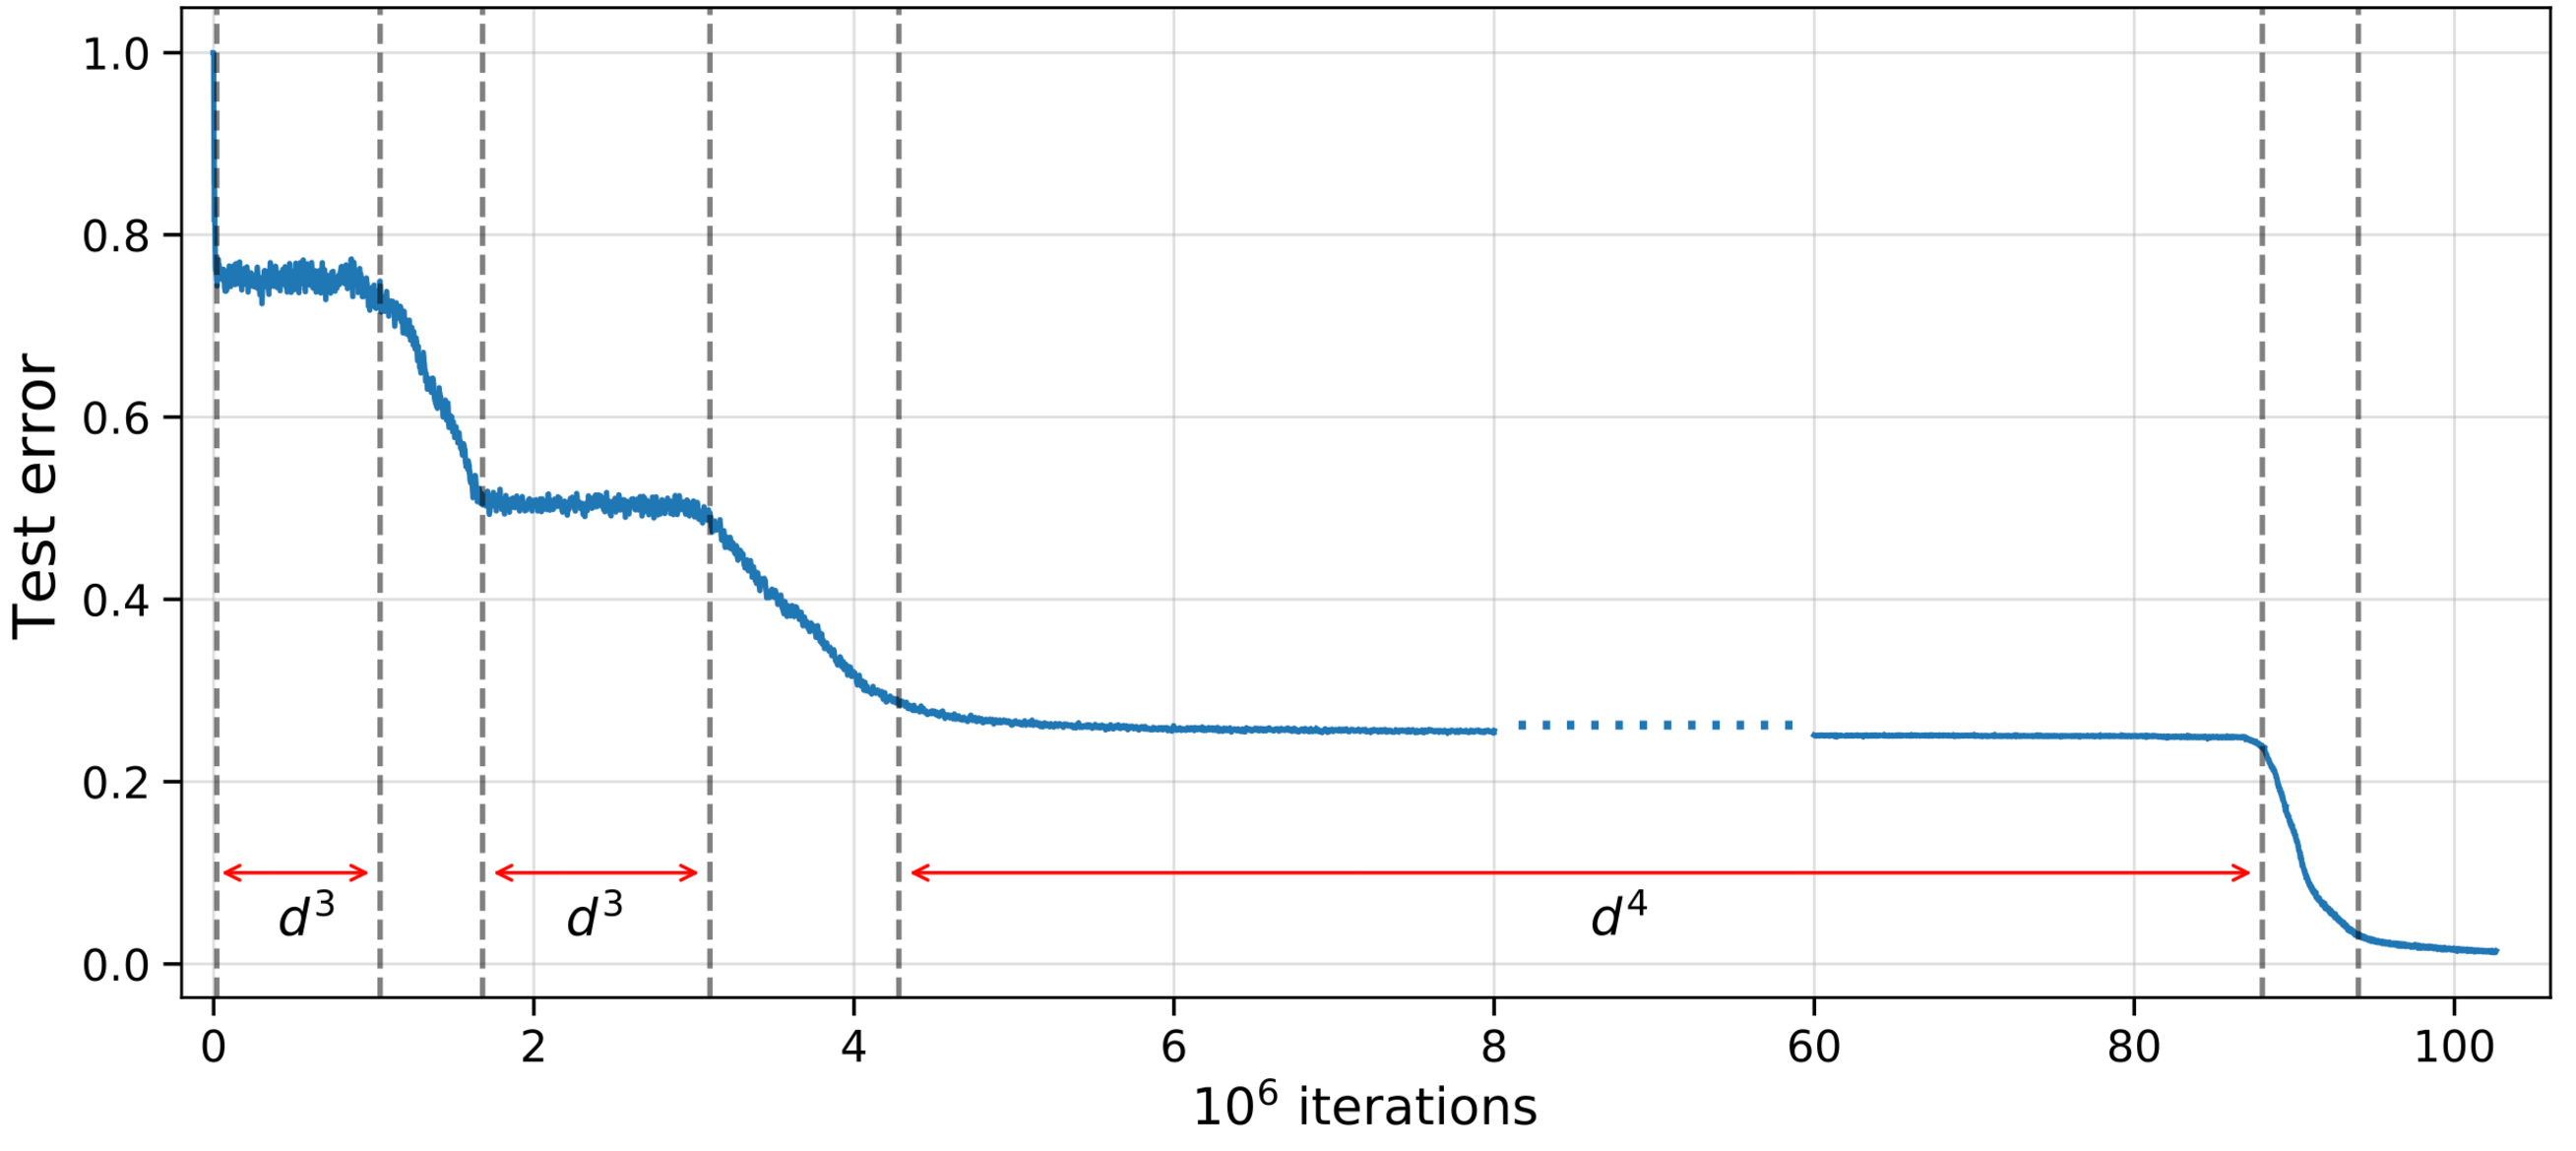
\includegraphics[width=0.90\textwidth]{assets/SaddleToSaddleSimu.pdf}
    \end{figure}

    \pause

    Saddle-to-saddle dynamics \citep{pesme2023saddle, abbe2023saddle} cause
    \bad{plateaus} in training loss and then
    \good{sudden drops} when the iterates escape.

    \source{https://arxiv.org/abs/2302.11055}

\end{frame}

\begin{frame}{Introduction: Flat Loss Surfaces}

    Faster optimization requires \good{escaping flat regions} quickly.

    \pause

    \begin{figure}[]
        \centering
        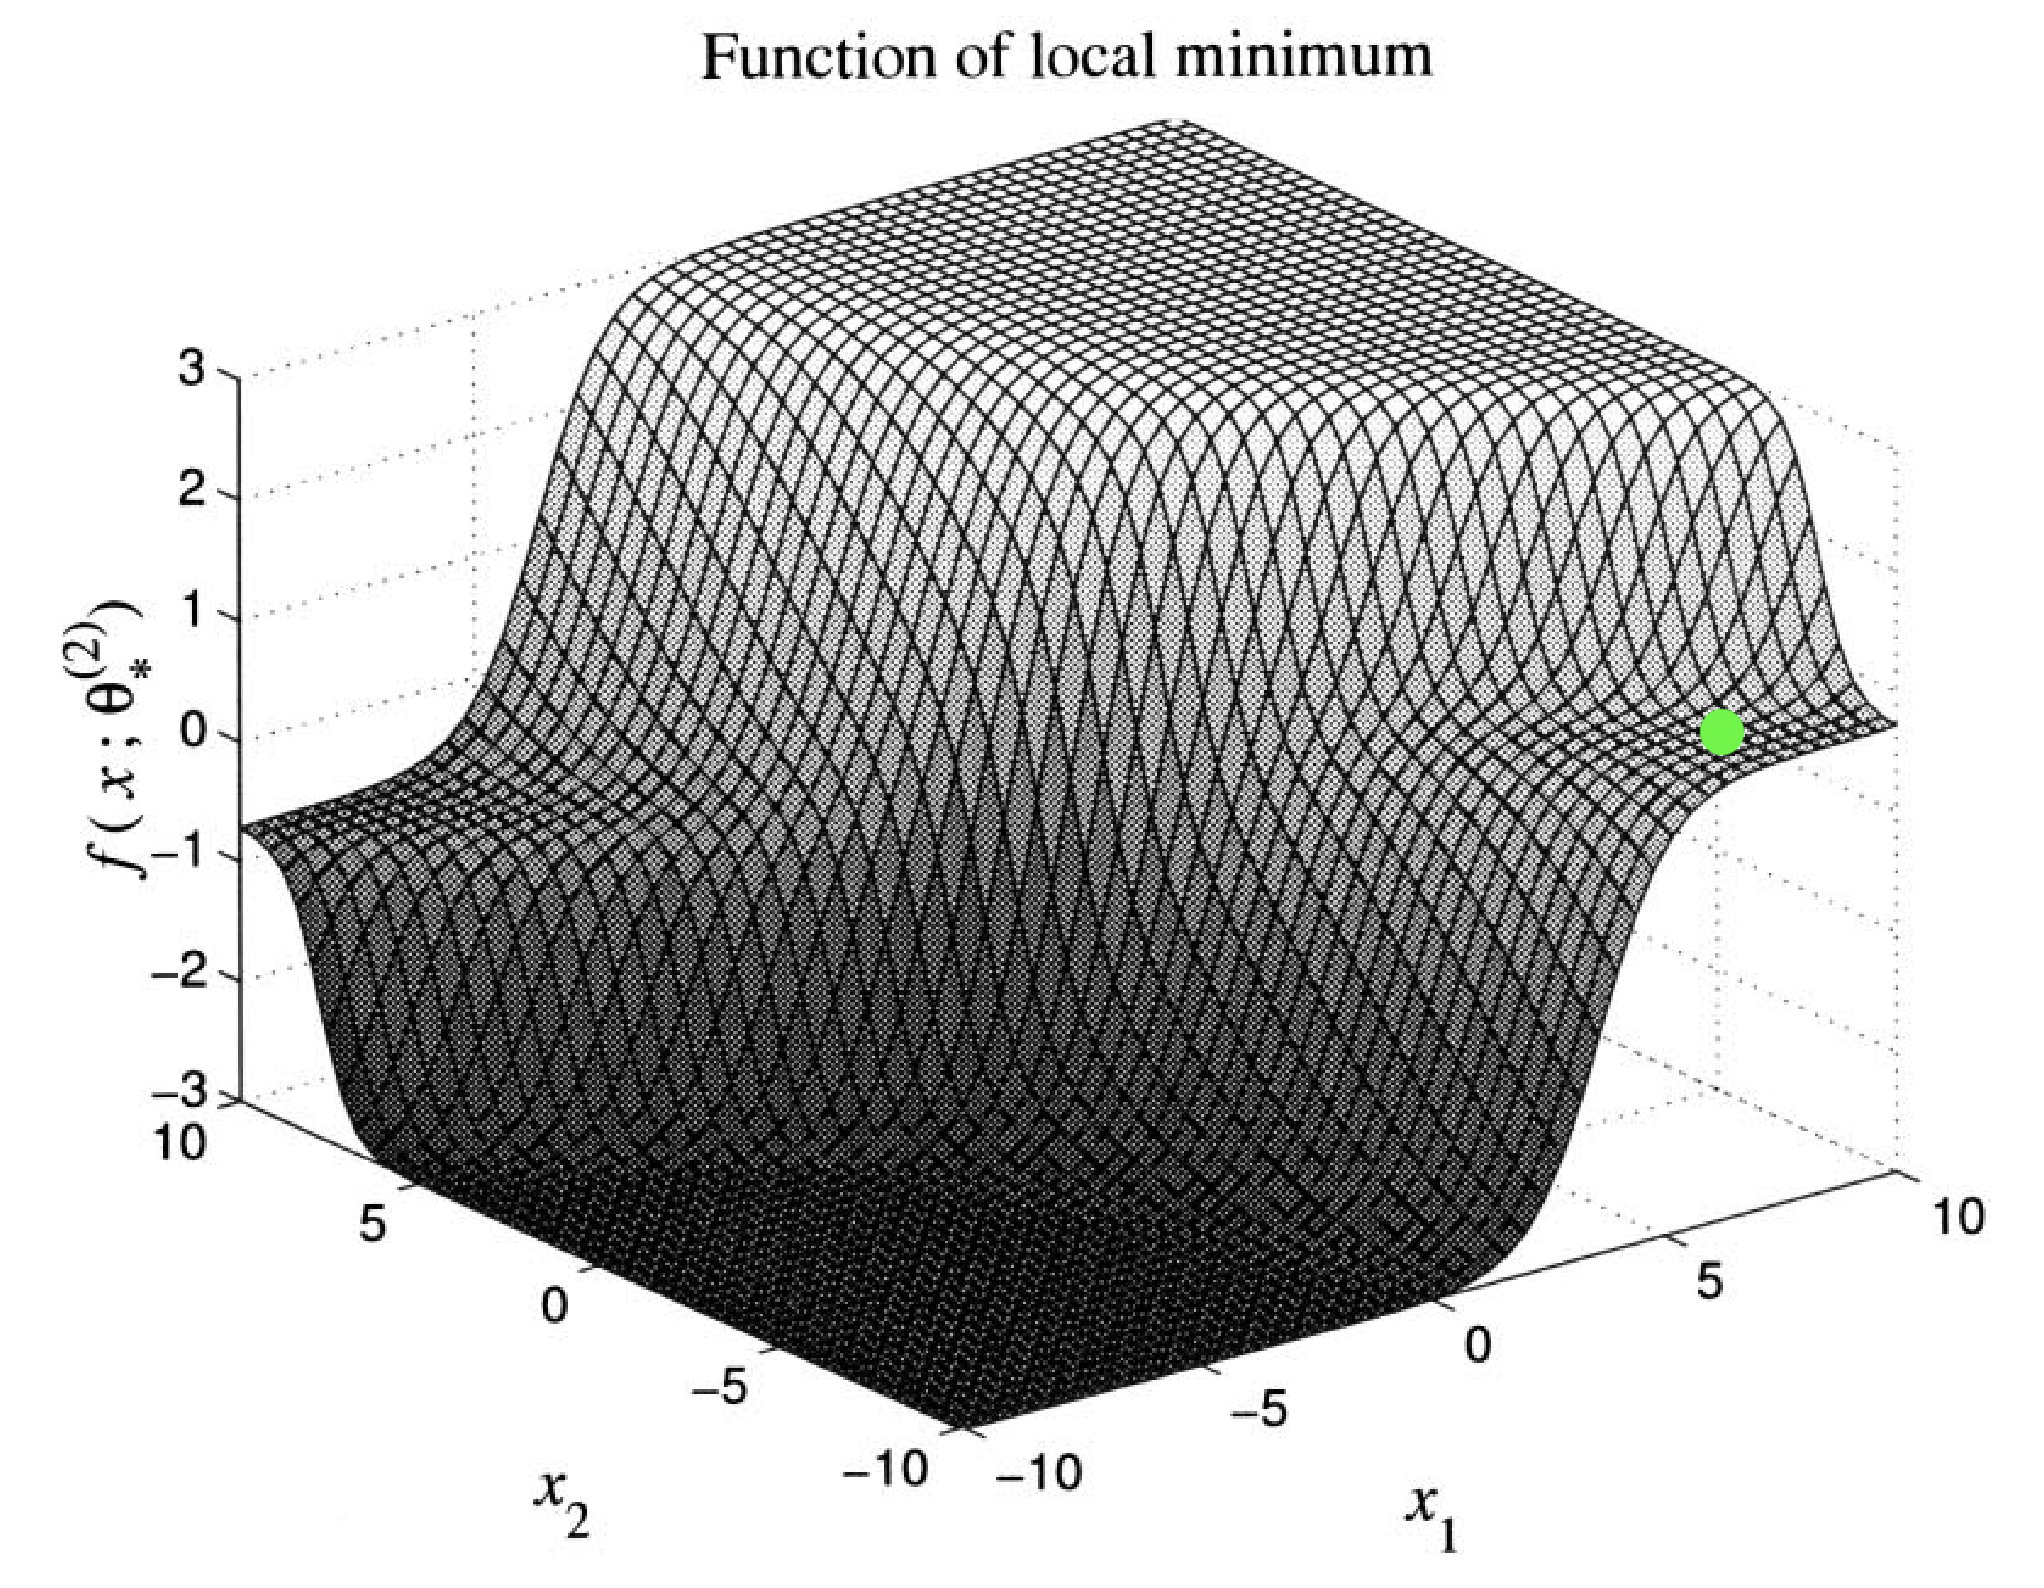
\includegraphics[width=0.7\textwidth]{assets/loss_surface_plain.png}
    \end{figure}

    \pause

    \begin{itemize}
        \item Newton's method could do this, but Newton doesn't work
              for non-convex objectives due to \bad{negative curvature}.
    \end{itemize}

    \source{https://www.sciencedirect.com/science/article/abs/pii/S0893608000000095}

\end{frame}

\begin{frame}{Introduction: Towards Teleportation}

    What we really want to do is \good{jump away} to a big gradient!

    \pause

    \begin{figure}[]
        \centering
        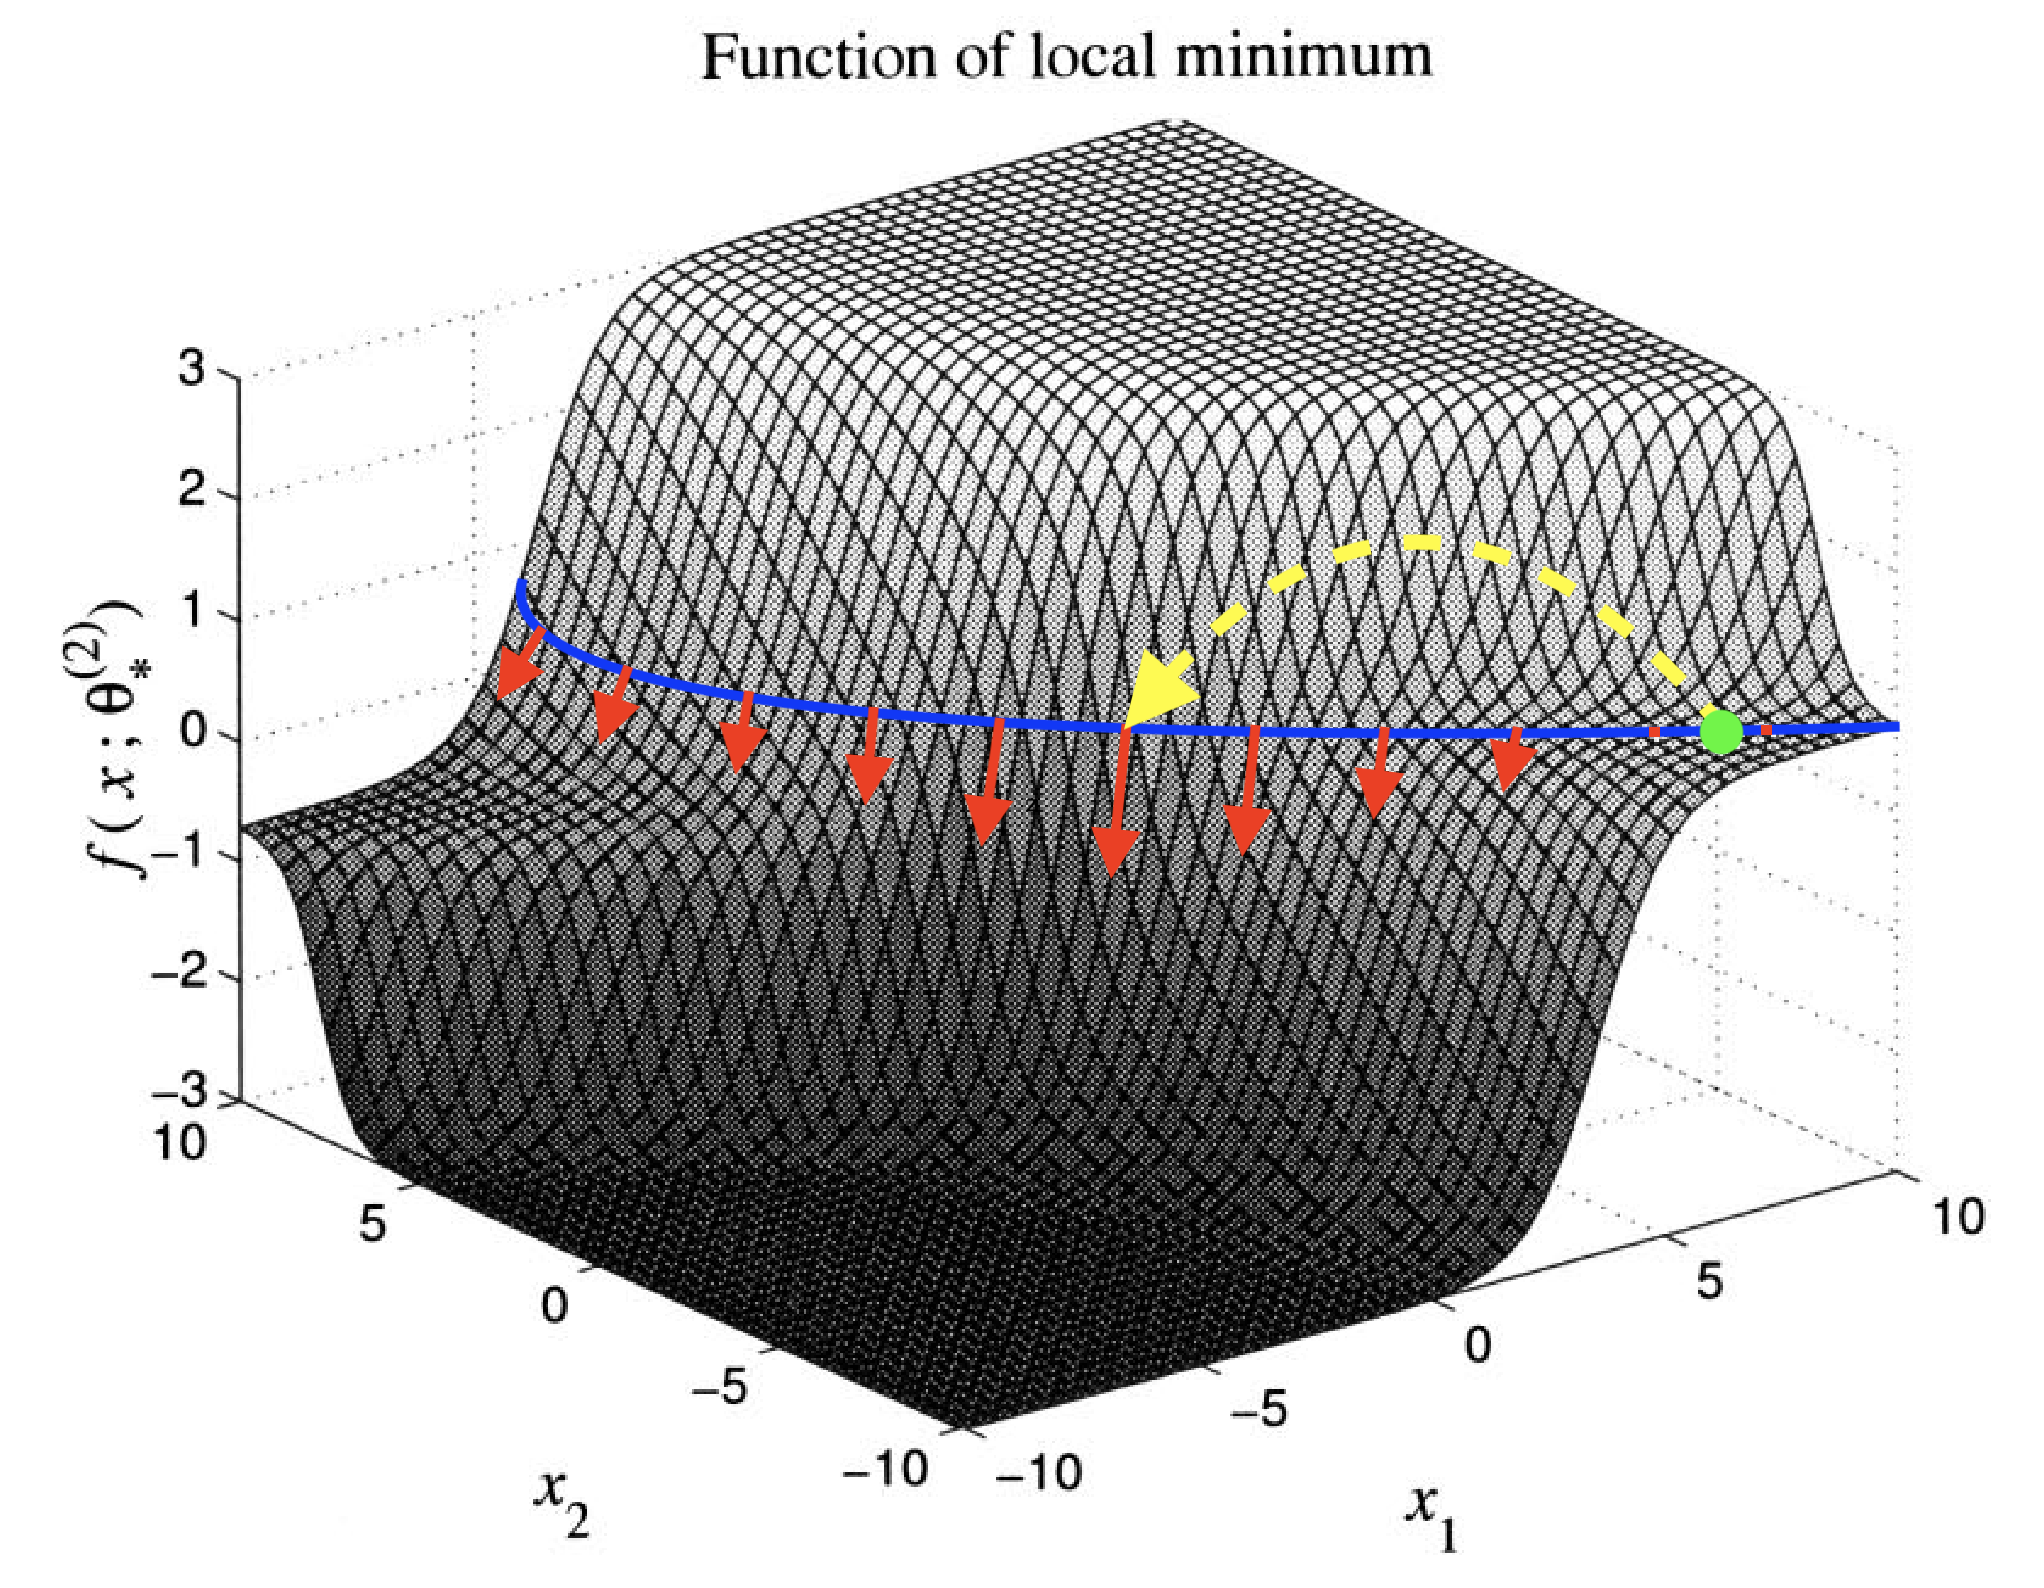
\includegraphics[width=0.7\textwidth]{assets/loss_surface_teleport.png}
    \end{figure}

    \pause

    This is the picture  behind \textbf{level set teleportation} \citep{zhao2023symmetry}.

    \source{https://www.sciencedirect.com/science/article/abs/pii/S0893608000000095}

\end{frame}

\begin{frame}{Introduction: Background}

    \textbf{Teleport incipit}:
    \citet{armenta2020neural, armenta2021representation}
    propose \good{random jumps} using symmetry operators.

    \pause
    \vspace{1ex}

    \begin{itemize}
        \item But it \bad{doesn't work} very well\ldots
    \end{itemize}

    \pause
    \horizontalrule

    \textbf{Enter optimization}:
    \citet{zhao2023improving} \good{optimize} over symmetries and
    alternate between GD and teleportation steps.

    \pause
    \vspace{1ex}

    \begin{itemize}
        \item They use Newton's method to prove a \good{mixed linear/quadratic}
              rate for strongly-convex functions.
              \pause
              \vspace{1ex}

        \item They give standard rates under the PL-condition
              \citep{karimi2016pl} and slightly \good{stronger guarantees} for
              non-convex functions.
              \pause
              \vspace{1ex}

        \item But, symmetries only \bad{approximate teleportation}\ldots

              \pause
              \vspace{1ex}

        \item And nothing is known for \bad{non-strongly convex} functions.
              \pause
    \end{itemize}

    \vspace{2ex}

\end{frame}

\begin{frame}{Introduction: Contributions}
    \begin{figure}[]
        \centering
        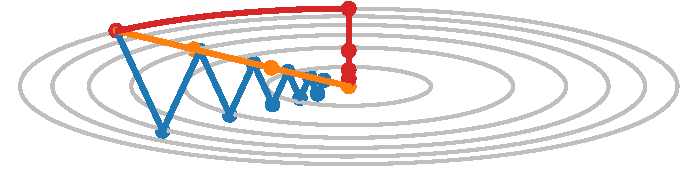
\includegraphics[width=0.9\textwidth]{assets/GD_combined.pdf}
    \end{figure}

    \textbf{Our Contributions}:
    \pause
    \begin{itemize}
        \item We show teleportation only accelerates optimization when (i)
              there is \bad{curvature} and (ii) \bad{adaptive step-sizes} are
              used.
              \pause
              \vspace{1ex}

        \item We show teleportation \good{speeds-up} optimization under Hessian
              stability (rates faster than \( O(1/K) \)!).
              \pause
              \vspace{1ex}

        \item We develop a \good{fast, parameter-free} algorithm for solving
              teleportation problems.
    \end{itemize}

\end{frame}

\setbeamercolor{background canvas}{bg=LightCyan}
\begin{frame}{}
    \begin{center}
        \huge Optimization Background
    \end{center}
\end{frame}
\setbeamercolor{background canvas}{bg=white}

\begin{frame}{Optimization Setting}

    \textbf{Goal}: minimize an \bad{objective} \( f : \R^d \into \R\),
    \[
        \calW^* = \argmin_{w} f(w).
    \]
    \pause

    We are willing to make the following assumptions.
    \vspace{1ex}
    \pause
    \begin{itemize}
        \item \( f \) is \good{convex}, meaning for every \( y, x \in \R^d\),
              \[
                  f(y) \geq f(x) + \abr{\grad(x), y - x}.
              \]
              \pause
              \vspace{-1ex}

        \item \( f \) is \good{differentiable} and
              \good{\( L \)-Smooth}: \( \forall x, y \in \R^d \),
              \[
                  \norm{\grad(y) - \grad(x)}_2 \leq L \norm{y - x}_2,
              \]
              \pause

              \vspace{-2ex}
              \begin{itemize}
                  \item \( \grad \) doesn't change \bad{too fast}\ldots
              \end{itemize}
    \end{itemize}
\end{frame}

\begin{frame}{Smoothness: Motivation}
    \begin{center}
        \Large
        Why do we need \( \grad \) to be \( L \)-Smooth?
    \end{center}

    \pause
    \horizontalrule

    \textbf{Intuition}: gradient magnitude isn't informative for non-smooth \( f \).
    \[
        \textbf{GD}: \, \wkk = \wk - \eta \grad(\wk).
    \]
    \pause

    \vspace{2ex}

    \begin{center}
        %! TEX root = ../../main.tex

%% Illustration of cone decomposition. 

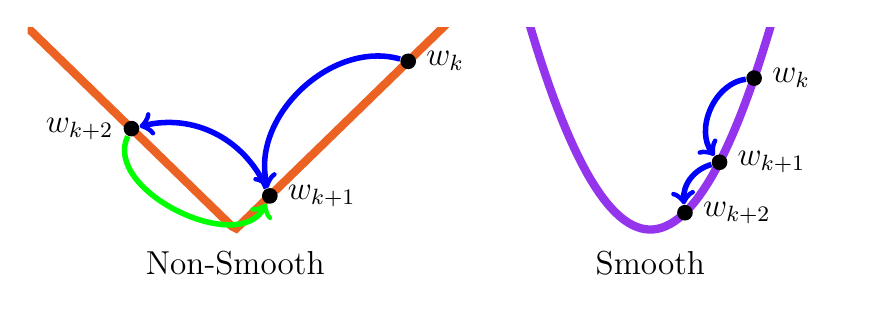
\begin{tikzpicture}[scale=1,
		declare function={
				abs_off(\x)= 2*abs(x + 3);
				quad_off(\x)= 2*(x - 3)^2;
			}
	]
	\begin{axis}[width=\linewidth, height=5cm,
			axis lines=none, yticklabels={,,}, xticklabels={,,},
			ymin=-2, ymax=6, ytick={0,...,5}, ylabel=$$, x axis line style={-},
				xmin=-6, xmax=6, xtick={-5,...,5}, xlabel=$$, y axis line style={-},
		]

		\addplot[name path=abs, domain=-6:6, samples=200, line width=3pt, color=bad, visible on=<3->]{abs_off(x)};
		\node[visible on=<3->] at (axis cs:-3,-1) {Non-Smooth};

		\node[name=aw1, label={[visible on=<4->]right:$\wk$}, circle, fill, inner sep=2pt, visible on=<4->] at (axis cs:-0.5,5) {};
		\node[name=aw2, label={[visible on=<5->]right:$w_{k+1}$}, circle, fill, inner sep=2pt, visible on=<5->] at (axis cs:-2.5,1) {};
		\node[name=aw3, label={[visible on=<6->]left:$w_{k+2}$}, circle, fill, inner sep=2pt, visible on=<6->] at (axis cs:-4.5,3) {};

		\draw [->, line width=2pt, bend right=60, color=blue, visible on=<5->] (aw1) to (aw2);
		\draw [->, line width=2pt, bend right=40, color=blue, visible on=<6->] (aw2) to (aw3);
		\draw [->, line width=2pt, bend right=90, color=green, visible on=<7->] (aw3) to (aw2);


		\addplot[name path=quad, domain=-6:6, samples=200, line width=3pt, color=good, visible on=<8->]{quad_off(x)};
		\node[visible on=<8->] at (axis cs:3,-1) {Smooth};

		\node[name=qw1, label={[visible on=<9->]right:$\wk$}, circle, fill, inner sep=2pt, visible on=<9->] at (axis cs:4.5,4.5) {};
		\node[name=qw2, label={[visible on=<10->]right:$\wkk$}, circle, fill, inner sep=2pt, visible on=<10->] at (axis cs:4,2) {};
		\node[name=qw3, label={[visible on=<11->]right:$w_{k+2}$}, circle, fill, inner sep=2pt, visible on=<11->] at (axis cs:3.5,0.5) {};

		\draw [->, line width=2pt, bend right=60, color=blue, visible on=<10->] (qw1) to (qw2);
		\draw [->, line width=2pt, bend right=40, color=blue, visible on=<11->] (qw2) to (qw3);

		%\draw [name path=cone_1, solid, line width=1pt] (axis cs:0,-2) -- (axis cs:0,6);
		%\draw [name path=bounds, line width=0pt] (axis cs:6,-2) -- (axis cs:6,6);
		%\tikzfillbetween[of=cone_1 and bounds, on layer=ft]{good, opacity=0.1};

		%%% point labels
		%% origin point
		%\node[circle, fill, inner sep=1pt] at (axis cs:0,0) {};

		%% active examples 
		%\node[label=right:$(x_1\!\mathbin{,} y_1)$, circle, draw, line width=0.25mm, inner sep=0.5mm] at (axis cs:-5,1) {};
		%\node[label=right:$(x_2\!\mathbin{,} y_2)$, circle, fill, inner sep=0.5mm] at (axis cs:0.5,5) {};


		%% lines
		%\draw [->, draw=bad, line width = 1mm] (axis cs:0,0) -- (axis cs:5,0) node[near end,above right] {$w^*_{1}$};

		%\node[] at (axis cs:-4,5) { $ \lambda \approx 0$ };
	\end{axis}

\end{tikzpicture}%
%
    \end{center}

\end{frame}

\begin{frame}{Back to Level Set Teleportation}

    \textbf{Basic Idea}: \( L \)-smoothness relates
    gradient magnitude to progress in function values via the
    \emph{descent lemma},
    \[
        f(\wkk) \leq f(\wk) - \inv{L}\norm{\grad(\wk)}_2^2.
    \]
    \pause

    \begin{itemize}
        \item All other quantities \bad{held constant}, maximizing \(
              \norm{\grad(\wk)}_2 \) maximizes \good{guaranteed progress}.
    \end{itemize}

    \pause
    \horizontalrule
    \vspace{2ex}

    Now we can give a formal version of ``jumping to big gradients'':
    \pause
    \[
        \textbf{Teleport: } \wk^+ \in \argmax_w \, \half \norm{\grad(w)}^2_2  \quad \text{s.t.} \quad f(w) \leq f(\wk).
    \]

\end{frame}

\setbeamercolor{background canvas}{bg=LightCyan}
\begin{frame}{}
    \begin{center}
        \huge Level Set Teleportation
    \end{center}
\end{frame}
\setbeamercolor{background canvas}{bg=white}

\begin{frame}{Level Set Teleportation: Algorithm}

    \begin{itemize}
        \item Let \( \calB \subset \bbN \) be \good{start indices} for teleportation
              blocks.
              \pause

        \item Each \good{teleportation block} \( i \in \calB \) consists of \( b_i \geq 1 \)
              steps.
              \pause

        \item Complete \good{teleportation schedule} is \( \calT \).
    \end{itemize}
    \pause

    \begin{algorithm}[H]
        \caption{GD with Teleportation}
        \label{alg:gd-with-teleport}
        \begin{algorithmic}
            \STATE \textbf{Inputs}: \( w_0 \); step-sizes \( \etak \); block indices \( \calB \), sizes \( b_k \).
            \STATE \( \calT \gets \bigcup_{k \in \calB} \cbr{k, k+1, \ldots, k+b_k-1} \)
            \FOR{\( k \in \cbr{0, \ldots, K} \)}
            \IF{\( k \in \calT \)}
            \STATE \( w_k^+ \in \argmax \cbr{\norm{\grad(w)}_2 : f(w) \leq f(\wk)} \)
            \ELSE
            \STATE \( w_k^+ \gets w_k \)
            \ENDIF
            \STATE \( \wkk \gets \wk^+ - \etak \grad(\wk^+) \)
            \ENDFOR
            \STATE \textbf{Output}: \( w_K \)
        \end{algorithmic}
    \end{algorithm}
\end{frame}

\begin{frame}{Level Set Teleportation: Test Functions}

    \[
        \wk^+ \in \argmax_w \, \half \norm{\grad(w)}^2_2  \quad \text{s.t.} \quad f(w) \leq f(\wk).
    \]

    \horizontalrule
    \pause

    \begin{figure}[]
        \centering
        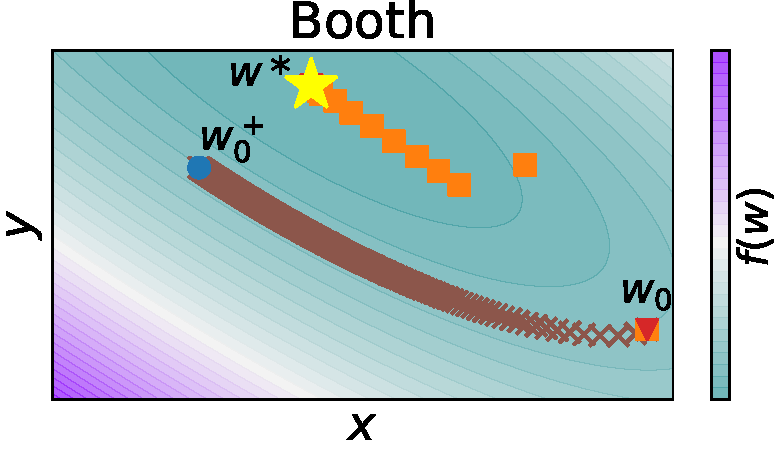
\includegraphics[width=0.49\textwidth]{assets/Booth-2d.pdf}
        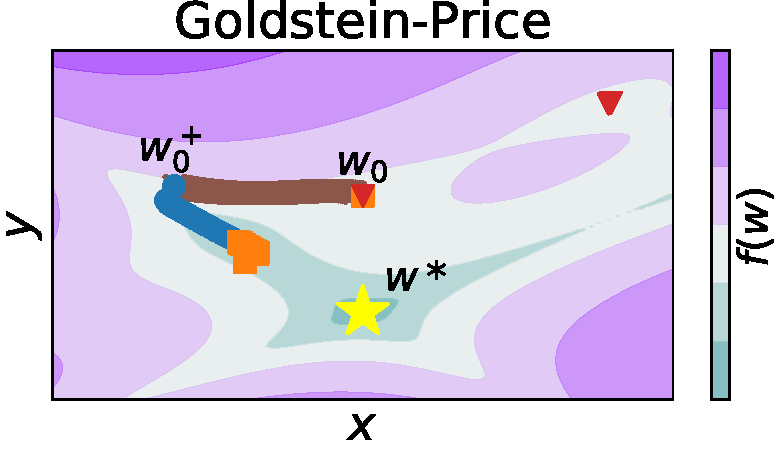
\includegraphics[width=0.49\textwidth]{assets/Goldstein-Price-2d.pdf}
    \end{figure}

    \begin{center}
        \Large Teleportation in action on two test functions.
    \end{center}
\end{frame}

\begin{frame}{Level Set Teleportation: Faster Descent}
    \textbf{GD with teleportation}:
    \[
        \begin{aligned}
            \wk^+ & \in \argmax_w \, \half \norm{\grad(w)}^2_2  \quad \text{s.t.} \quad f(w) \leq f(\wk) \\
            \wkk  & = \wk - \etak \grad(\wk^+).
        \end{aligned}
    \]

    \pause
    \horizontalrule

    We can derive a \good{tighter descent lemma} for steps with teleportation!
    \pause
    \vspace{-1ex}

    \begin{align*}
        f(\wkk)
         & \leq f(\wk^+) - \etak (1 - \frac{\etak L}{2}) \norm{\grad(\wk^+)}_2^2                          \\
         & \leq f(\wk) - \etak (1 - \frac{\etak L}{2}) \max \cbr{\norm{\grad(w)}_2^2 : f(w) \leq f(\wk)}.
    \end{align*}
    \pause
    \vspace{-1ex}

    This approach leads to standard \( O(1/T) \) convergence, but on
    the \good{maximum} gradient \( \max \cbr{\norm{\grad(w)}_2^2 : f(w) \leq f(\wk)} \)
    \citep{zhao2023symmetry}.

\end{frame}

\begin{frame}{Level Set Teleportation: Newton's Method}

    \[
        \wk^+ \in \argmax_w \, \half \norm{\grad(w)}^2_2  \quad \text{s.t.} \quad f(w) \leq f(\wk).
    \]

    \pause
    \horizontalrule

    \begin{itemize}

        \item If \( \grad(\wk) \neq 0 \), then the KKT conditions are
              \good{necessary} for \( \wk^+ \) to be
              a local maximum:
              \[
                  \nabla^2 f(\wk^+) \grad(\wk^+) - \lambda_k \grad(\wk^+) = 0.
              \]
              \pause
              \vspace{-3ex}

        \item \( \lambda_k \) is an eigenvalue of \( \nabla^2 f(\wk^+) \) and
              if \( \lambda_k \neq 0 \), then
              \[
                  \grad(\wk^+) = \lambda_k \sbr{\nabla^2 f(\wk^+)}^{\dagger} \grad(\wk^+).
              \]
              \pause

        \item The gradient direction is the \emph{Newton direction} with scale \( \lambda_k \)!

    \end{itemize}
\end{frame}

\begin{frame}{Level Set Teleportation: Strong Convexity}
    \textbf{Strong Convexity}: \( f \) is \( \mu \)-SC if for all \( x,y \in \R^d \),
    \[
        f(y) \geq f(x) + \abr{\grad(x), y - x} + \frac{\mu}{2} \norm{y - x}_2^2.
    \]
    \pause
    \vspace{-2ex}

    Ensures \( \nabla^2 f(\wk) \) is P.D.\ and \( \lambda_k > 0 \).
    \pause
    \horizontalrule

    \citet{zhao2023improving} use this to analyze GD with teleportation.
    \pause
    \vspace{1em}
    \begin{itemize}
        \item This approach leads to standard, \good{super-linear} rates using
              Newton-type analyses.

              \pause
              \vspace{1em}
        \item But it requires teleporting before \bad{every iteration} of GD
              and \bad{strong convexity} is key.
    \end{itemize}

\end{frame}

\begin{frame}{Level Set Teleportation: More Problems}

    And there are some more \bad{problems}\ldots

    \vspace{2ex}
    \pause

    \begin{enumerate}
        \item Teleportation can \bad{blow-up} the distance to a minimizer,
              \[
                  \norm{\wk^+ - \wopt}_2 \geq \bad{C} \norm{\wk - \wopt}.
              \]
              \vspace{-2ex}
              \pause
              \begin{itemize}
                  \item Breaks standard proof techniques for non-strongly convex \( f \).
              \end{itemize}

              \pause
              \vspace{2ex}

        \item If \( f \) is non-strongly convex, then \( \nabla^2 f(\wk) \) can
              be positive \bad{semi}-definite and \bad{\( \lambda_k = 0 \)} may happen.
              \vspace{1ex}
              \pause
              \begin{itemize}
                  \item Breaks the connection to Newton's method.
              \end{itemize}

              \pause
              \vspace{2ex}

        \item No efficient algorithms for \bad{teleporting in practice}!
    \end{enumerate}

\end{frame}

\setbeamercolor{background canvas}{bg=LightCyan}
\begin{frame}{}
    \begin{center}
        \huge Analysis and Algorithms
    \end{center}
\end{frame}
\setbeamercolor{background canvas}{bg=white}

\begin{frame}{Convergence Analysis: Convex Functions}

    \begin{center}
        \large
        \textbf{Goal}: fast rates for GD with \emph{intermittent} teleportation.
    \end{center}

    \horizontalrule
    \pause

    The key to faster rates is the \good{KKT} stationarity condition,
    \[
        \grad(\wk^+) = \lambda_k \sbr{\nabla^2 f(\wk^+)}^{\dagger} \grad(\wk^+).
    \]

    \pause
    \vspace{2ex}

    \begin{itemize}
        \item But we can't use this because \bad{$\lambda_k > 0$} may not hold\ldots

              \pause
              \vspace{2ex}

        \item \bad{Worse}, \( \norm{\wk^+ - \wopt}_2^2 > \bad{C} \norm{\wk - \wopt}_2^2 \)
              breaks standard proofs:
              \[
                  \begin{aligned}
                      \norm{\wkk - \wopt}_2^2
                       & =
                      \norm{\wk^+ - \wopt}_2^2 \\
                       & \hspace{1em}
                      - 2 \etak \abr{\grad(\wk^+), \wk^+ - \wopt}
                      + \etak^2 \norm{\grad(\wk^+)}_2^2,
                  \end{aligned}
              \]
    \end{itemize}

\end{frame}

\begin{frame}{Convergence Analysis: Convex Functions}

    \good{Solution}: Teleportation is non-expansive in function values,
    \[
        f(\wkk) \leq f(\wk^+) \leq f(\wk).
    \]
    \pause%
    As a result, all iterates remain in the initial sub-level set
    \[
        \calS_0 := \cbr{w : f(w) \leq f(w_0)}.
    \]
    \vspace{-2ex}
    \pause

    \begin{theorem}[Informal]
        Let \( R = \sup \cbr{\norm{w - \wopt}_2 : w \in \calS_0 } \).
        If \( f \) is \( L \)-smooth and convex,
        then GD with \( \eta < 2 / L \) and
        teleportation schedule \( \calT \) satisfies,
        \[
            f(w_K) - f(\wopt) \leq \frac{2 R^2}{K \eta \rbr{2 - L \eta}}.
        \]
        Moreover, there exists a function for which the convergence of GD
        with and without teleportation are identical.
    \end{theorem}

    \pause
    This is similar to the strategy used by \citet{beck2013bcd}.
\end{frame}

\begin{frame}{Convergence: A Negative Tightness Result}
    Denote \( \delta_K = f(\w_K) - f(\wopt) \).
    Comparing to standard GD \citep{bubeck2015convex},
    \[
        \underbrace{
            \delta_K \leq \frac{2 \bad{R^2}}{K \eta \rbr{2 - L \eta}}
        }_{\text{With Teleportation}}
        \quad \textbf{vs} \quad
        \underbrace{
            \delta_K \leq \frac{2 \good{\norm{w_0 - \wopt}_2^2}}
            {K \eta \rbr{2 - L \eta}}.
        }_{\text{Without Teleportation}}
    \]

    \pause
    \vspace{2ex}

    Unfortunately, the dependence on the diameter is \bad{tight}.
    \vspace{1ex}
    \begin{theorem}[Informal]
        There exists an \( L \)-smooth and convex function
        such that teleporting from the initialization guarantees,
        \[
            \norm{\w_0^+ - \wopt}_2 \geq R / 4.
        \]
    \end{theorem}
\end{frame}

\begin{frame}{Convergence: Hessian Stability}
    We need the connection to \good{Newton's method} to prove fast rates.
    \pause
    \begin{itemize}
        \item \( \nabla^2 f(w) \) needs to be positive definite and
              well-behaved.
    \end{itemize}

    \pause
    \horizontalrule

    \begin{definition}[Hessian Stability \citep{gower2019subspace, karimireddy2018global}]%
        \label{def:hessian-stability}
        We say \( f \) has \( (\tL, \tmu) \)-stable Hessian
        over \( \calQ \subseteq \R^d \) if for every \( x, y \in \calQ \),\,
        \( \nabla^2 f(x) (y - x) \neq 0 \) and,
        \begin{align*}
            f(y)
             & \leq f(x) + \abr{\grad(x), y \!-\! x}
            + \frac{\tL}{2} \norm{y \!-\! x}^2_{\bad{\nabla^2 f(x)}},%
            \\
            f(y)
             & \geq f(x) + \abr{\grad(x), y \!-\! x}
            + \frac{\tmu}{2} \norm{y \!-\! x}^2_{\bad{\nabla^2 f(x)}}.%
        \end{align*}
    \end{definition}

    \pause
    Holds for practical problems, including logistic regression \citep{bach2010self}.

\end{frame}

\begin{frame}{Convergence: Main Theoretical Challenge}
    Intermittent teleportation gives \emph{two progress conditions}:

    \pause
    \vspace{1ex}

    \begin{itemize}
        \item \textbf{Steps with teleportation}
              obtain a \good{linear rate} under Hessian stability via the
              connection to Newton's method,
              \[
                  f(\wkk) - f(\wopt) \leq (1 - \frac{\tmu}{\tL}) (f(\wk) - f(\wopt).
              \]

              \pause

        \item \textbf{Steps without teleportation} obtain a standard
              descent lemma leading to a \bad{sub-linear rate},
              \[
                  f(\wkk) - f(\wopt) \leq f(\wk) - f(\wopt)
                  - \frac{1}{2L} \norm{\grad(\wk)}_2^2.
              \]
    \end{itemize}
    \pause

    \horizontalrule

    Combining the two leads to tighter rates for teleportation!
    \pause

    \[
        f(w_{k + b_k}) - f(\wopt) \leq (1 - \frac{\tmu}{\tL})^{b_k} \sbr{f(w_{k-1}) - f(\wopt) - \frac{1}{2L} \norm{\grad{w_{k-1}}}_2^2}.
    \]

\end{frame}

\begin{frame}{Convergence: Fast Rates under Hessian Stability}
    Recall that \( \delta_k = f(\wk) - f(\wopt) \) is the optimality gap.
    \vspace{2ex}

    \pause

    \begin{theorem}[Informal]
        Suppose \( f \) is \( L \)-smooth, convex, and satisfies Hessian
        stability on \( \calS_0 \).
        Let \( M = K - \abs{\calT} \).
        Then GD with line-search satisfies,
        \begin{equation*}
            \delta_K \leq
            \frac{2 R^2 L}
            {\bad{M} + 2 R^2 L \sum_{k \in \calB}
                \good{\sbr{
                        \rbr{\frac{\tL}{\tL - \tmu}}^{b_k} - 1} \inv{\delta_{k-1}}
                }}.
        \end{equation*}
    \end{theorem}

    \pause

    \begin{center}
        \Large
        Convergence is faster than GD when \( \delta_{k} \) is small!
    \end{center}

\end{frame}

\begin{frame}{Convergence: Simplified Rates}

    \begin{itemize}
        \item An alternative proof technique makes this rate explicit.
              \pause
        \item Consider teleporting every other iteration:
              \( \calT = \cbr{1, 3, 5, \ldots} \).
    \end{itemize}
    \pause

    \begin{theorem}
        Suppose \( f \) is \( L \)-smooth, convex, and satisfies Hessian
        stability on \( \calS_0 \).
        Then GD with line-search satisfies,
        \begin{equation*}
            \delta_K
            \leq
            \frac{2 R^2 L (\tL - \tmu)}{\tmu \sbr{\rbr{\frac{\tL}{\tL - \tmu}}^{K/2} - 1}}
            \approx
            2 R^2 L \tilde C
            \good{\rbr{1 - \frac{\tmu}{\tL}}^{K/2}}.
        \end{equation*}
    \end{theorem}
    \pause

    \begin{center}
        \Large
        This is a linear rate without strong convexity!
    \end{center}

\end{frame}

\begin{frame}{Level Set Teleportation: Towards an Algorithm}

    \[
        \wk^+ \in \argmax_w \, \half \norm{\grad(w)}^2_2  \quad \text{s.t.} \quad f(w) \leq f(\wk).
    \]

    \horizontalrule
    \pause

    \textbf{Restrictions} on an efficient teleportation algorithm.

    \vspace{1ex}

    \begin{itemize}
        \item The derivative of the gradient norm is a
              \bad{Hessian-vector product}: \( \nabla^2 f(x) \grad(x) \).
              \pause
              \vspace{1ex}

        \item We can't use generic second-order solvers, since computing the
              Hessian requires
              \bad{third-order derivatives}.

              \pause
              \vspace{1ex}
        \item The algorithm must be \good{parameter-free} because
              teleportation is only a sub-routine of GD.
    \end{itemize}
    \pause
    \vspace{1ex}

    These constraints suggest \good{first-order methods}.

\end{frame}

\begin{frame}{Level Set Teleportation: Practical Teleportation}

    We can't project onto \( \calL_k := \cbr{w : f(w) = f(\wk)} \),
    but we can project onto the \good{linearization} at \( \xk \):
    \[
        l_k = \cbr{ w : f(\xk) + \abr{\grad(\xk), w - \xk} = f(\wk) }
    \]
    \pause
    \vspace{-4ex}

    \begin{center}
        %\hspace{-1.5em}
        \begin{tikzpicture}[scale=1,
	]
	\begin{axis}[width=1.1\linewidth, 
        height=0.6\linewidth,
        axis lines=none,  % don't print axis lines
        yticklabels={,,}, xticklabels={,,},
		ymin=-2, ymax=2, 
		xmin=-4, xmax=4,
		view={0}-{90},
		]

		\addplot3[
			domain=-4:4,
			domain y=-4:4,
			contour gnuplot={
                labels=false, 
                levels={1, 4, 10},
                draw color=black,
            },
            line width=2pt,
            samples=100,
		] {x^2 + 4*y^2 };

        \addplot[
            domain=-4:4,
            samples=10,
            line width=2pt,
            draw=red,
            ] {-x/2 + 2/sqrt(2)};

        \addplot[
            ->,
            domain=1.414:1.545,
            samples=10,
            line width=2pt,
            draw=blue,
            ] {8*x - 15/sqrt(2)};

        \addplot[
            domain=-4:4,
            samples=10,
            line width=2pt,
            draw=purple,
            ] {1.0227 + (4 - 2*0.783*(x-0.783) - 0.783^2 - 4*1.0227^2)/(8*1.0227)};

       \node[
           star,
           fill=black,
           inner sep=0pt,
           minimum size=6pt,
           label={[label distance=-1.0mm]90:{$\wopt$}}
           ] (opt) at (axis cs:0,0) {};

       \node[
           label={[label distance=2.2mm]90:{$F(\w)$}}
           ] at (axis cs:1,-0.5) {};

       \node[
           circle,
           fill=black,
           inner sep=0pt,
           minimum size=6pt,
           label={[label distance=-1mm]90:{$x_0$}}
           ] (a) at (axis cs:1.414,0.707) {};

       \node[
           circle,
           fill=black,
           inner sep=0pt,
           minimum size=6pt,
           label={[label distance=0mm]180:{$x_0^+$}}
           ] (b) at (axis cs:1.55,1.79) {};

       \node[
           circle,
           fill=black,
           inner sep=0pt,
           minimum size=6pt,
           label={[label distance=0mm]90:{$x_1$}}
           ] (c) at (axis cs:0.783,1.0227) {};

       \draw[
           ->, 
           draw=orange,
           line width=2pt,
           ] (b) -- (c);

       \node[
           label={[label distance=-1mm, text=red]90:{$l_0$}}
           ] at (axis cs:2.5,0.164) {};

       \node[
           label={[label distance=-1.0mm, text=purple]90:{$l_1$}}
           ] at (axis cs:-1.4,1.4) {};

       \draw[
           draw=none,
           ] (a) -- (b)
           node[pos=0.84, right, text=blue]{$\nabla^2 F(x_0) \nabla F(x_0)$};

       \draw[
           draw=none,
           ] (b) -- (c)
           node[pos=0.50, left, text=orange]{$v_{0}$};

       %\draw[
       %    ->, 
       %    draw=BurntOrange,
       %    line width=2pt,
       %    ] (axis cs:0,1) -- (axis cs:0, 0.04) node [text=BurntOrange, left, pos=0.35, distance=-2mm] {$\nabla F(x^*)$};

       %\node[
       %    star,
       %    fill=orange,
       %    inner sep=0pt,
       %    minimum size=10pt,
       %    label={[label distance=-3mm, text=orange]70:{$x^*$}}
       %    ] (c) at (axis cs:0,1) {};


		%\draw [decorate, line width = 0.6mm,
		%    decoration = {calligraphic brace}] (axis cs:2.1,0.707) --  (axis cs:2.25,1.79)
            %node[midway,right]{$v_\varepsilon(a)$};
	\end{axis}
\end{tikzpicture}%

    \end{center}

\end{frame}

\begin{frame}{Level Set Teleportation: Practical Teleportation}

    \begin{algorithm}[H]
        \caption{Sub-level Set Teleportation}
        \label{alg:teleport}
        \begin{algorithmic}
            \STATE \( \x_0 \gets \wk \)
            \STATE \( q_0 \gets \nabla^2 f(\x_0) \grad(\x_0) \)
            \WHILE{\( \norm{\bfP_t q_t}_2 > \epsilon \) or \( f(\xk) - f(\wk) > \delta \)}
            \STATE \( g_t \gets \norm{\grad(\xk)}_2^2 \)
            \STATE \( v_{t} \gets - \rbr{\rho \abr{q_t, \grad(\xk) } + f(\xk) - f(\wk)}_+ \grad(\xk) \)
            \STATE \( \xkk \gets \xk + (\rho \cdot q_t + v_t) / g_t \)
            \WHILE{\( \phi_{\gamma_t}(\xkk) > \half g_t + (\abr{q_t, v_t} - \rho \norm{q_{t}}_2^2) / g_t \)}
            \STATE \( \rho \gets \rho / 2 \)
            \STATE \( v_{t} \gets -\! \rbr{\rho \abr{q_t, \!\grad(\xk) } \!+\! f(\xk) \!-\! f(\wk)}_+ \!\grad(\xk) \)
            \STATE \( \xkk \gets \xk + (\rho \cdot q_t + v_t) / g_t \)
            \ENDWHILE
            \STATE \( q_{t+1} \gets \nabla^2 f(\xk) \grad(\xk) \)
            \STATE \( t \gets t+1 \)
            \ENDWHILE
            \STATE \textbf{Output}: \( \xkk \)
        \end{algorithmic}
    \end{algorithm}
\end{frame}

\setbeamercolor{background canvas}{bg=LightCyan}
\begin{frame}{}
    \begin{center}
        \huge Experiments
    \end{center}
\end{frame}
\setbeamercolor{background canvas}{bg=white}

\begin{frame}{Experiments: Evaluating the Algorithm}

    Consider teleportation for a \bad{non-convex} neural network.
    \begin{itemize}
        \pause
        \item We consider a two-layer MLP with \( 50 \) hidden units and soft-plus activations.
              \pause
        \item Dataset is \texttt{MNIST}.
    \end{itemize}
    \pause
    \horizontalrule

    \begin{figure}
        \centering
        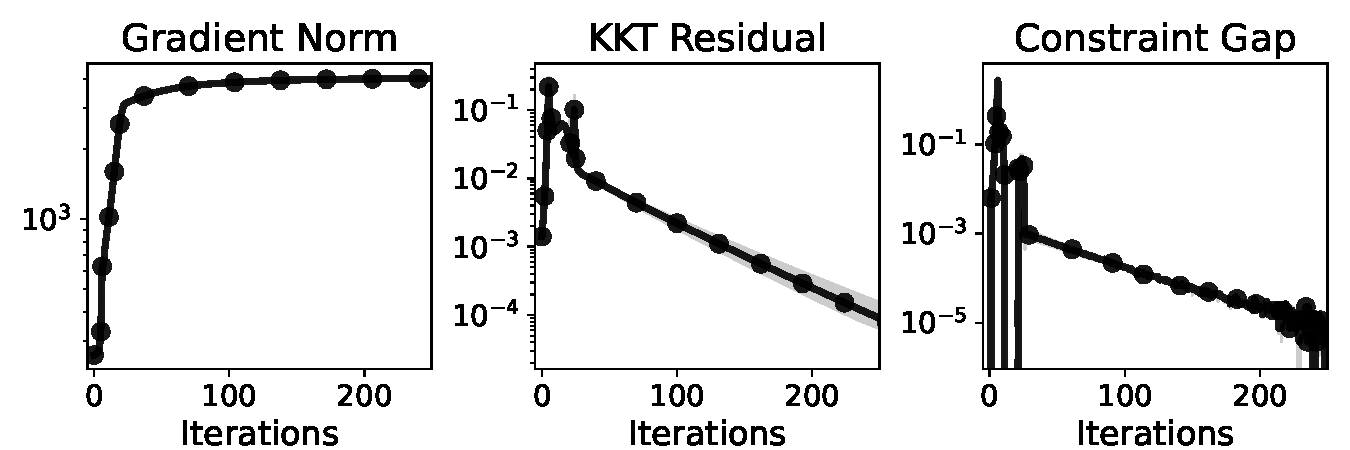
\includegraphics[width=0.99\textwidth]{assets/teleport_metrics_combined.pdf}
    \end{figure}

\end{frame}

\begin{frame}{Experiments: Performance Profile}

    We generate 120 problems from the UCI repository \citep{asuncion2007uci}.
    \begin{itemize}
        \pause
        \item Solid lines indicate methods \good{with teleportation}.
              \pause
        \item Dashed lines are the same methods \bad{without teleportation}.
    \end{itemize}
    \pause

    \begin{figure}
        \centering
        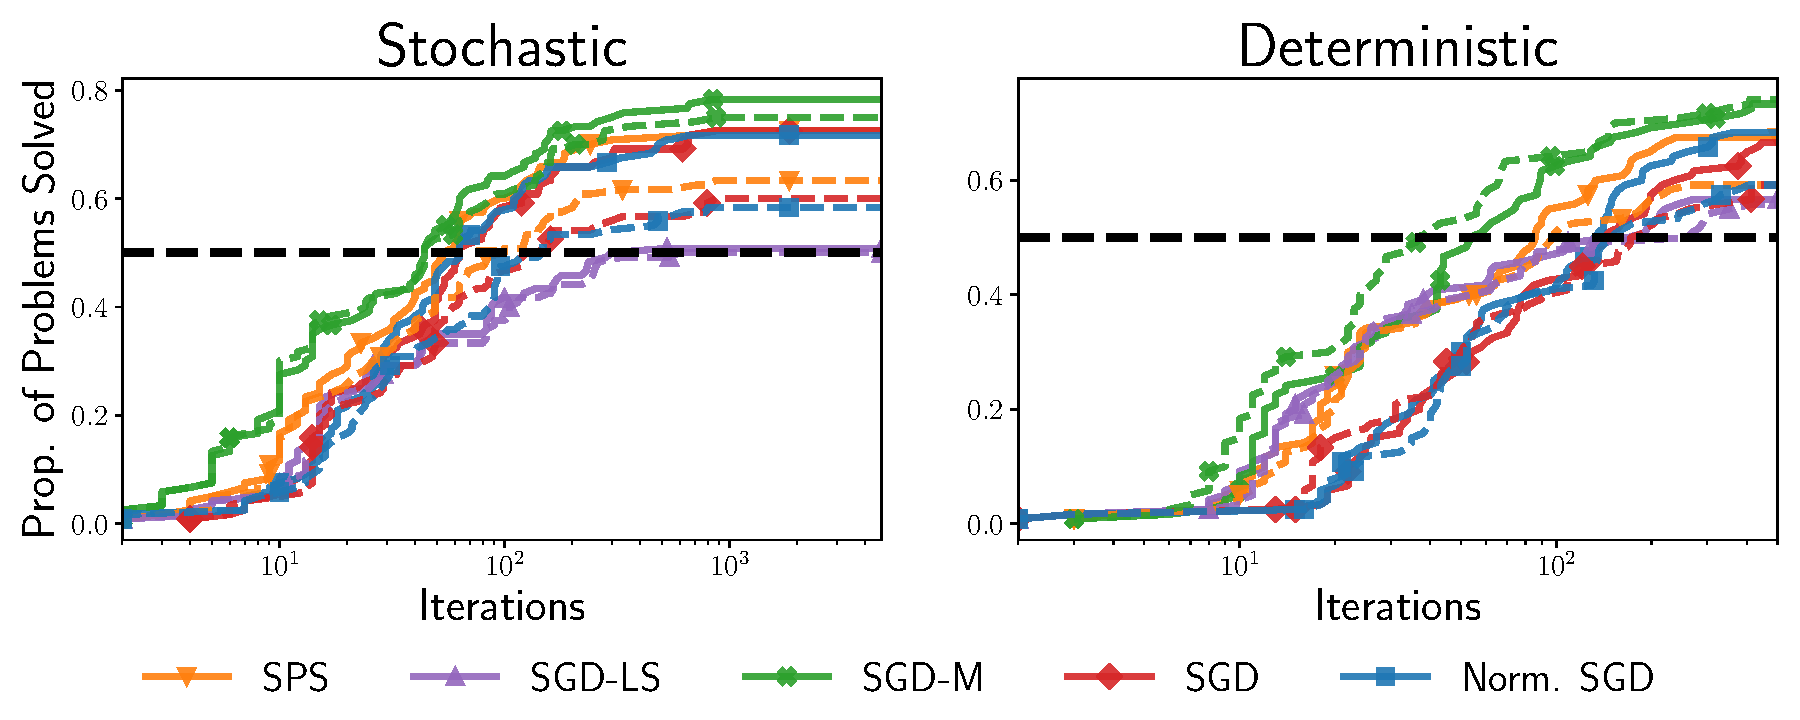
\includegraphics[width=1.0\textwidth]{assets/network_profile.pdf}
    \end{figure}

    \pause

    Teleportation \good{uniformly improves} speed and success rates!
\end{frame}

\begin{frame}{Experiments: Convex Newton}

    Teleporting at every iteration behaves like \bad{Newton's method}.

    \pause

    \begin{figure}
        \centering
        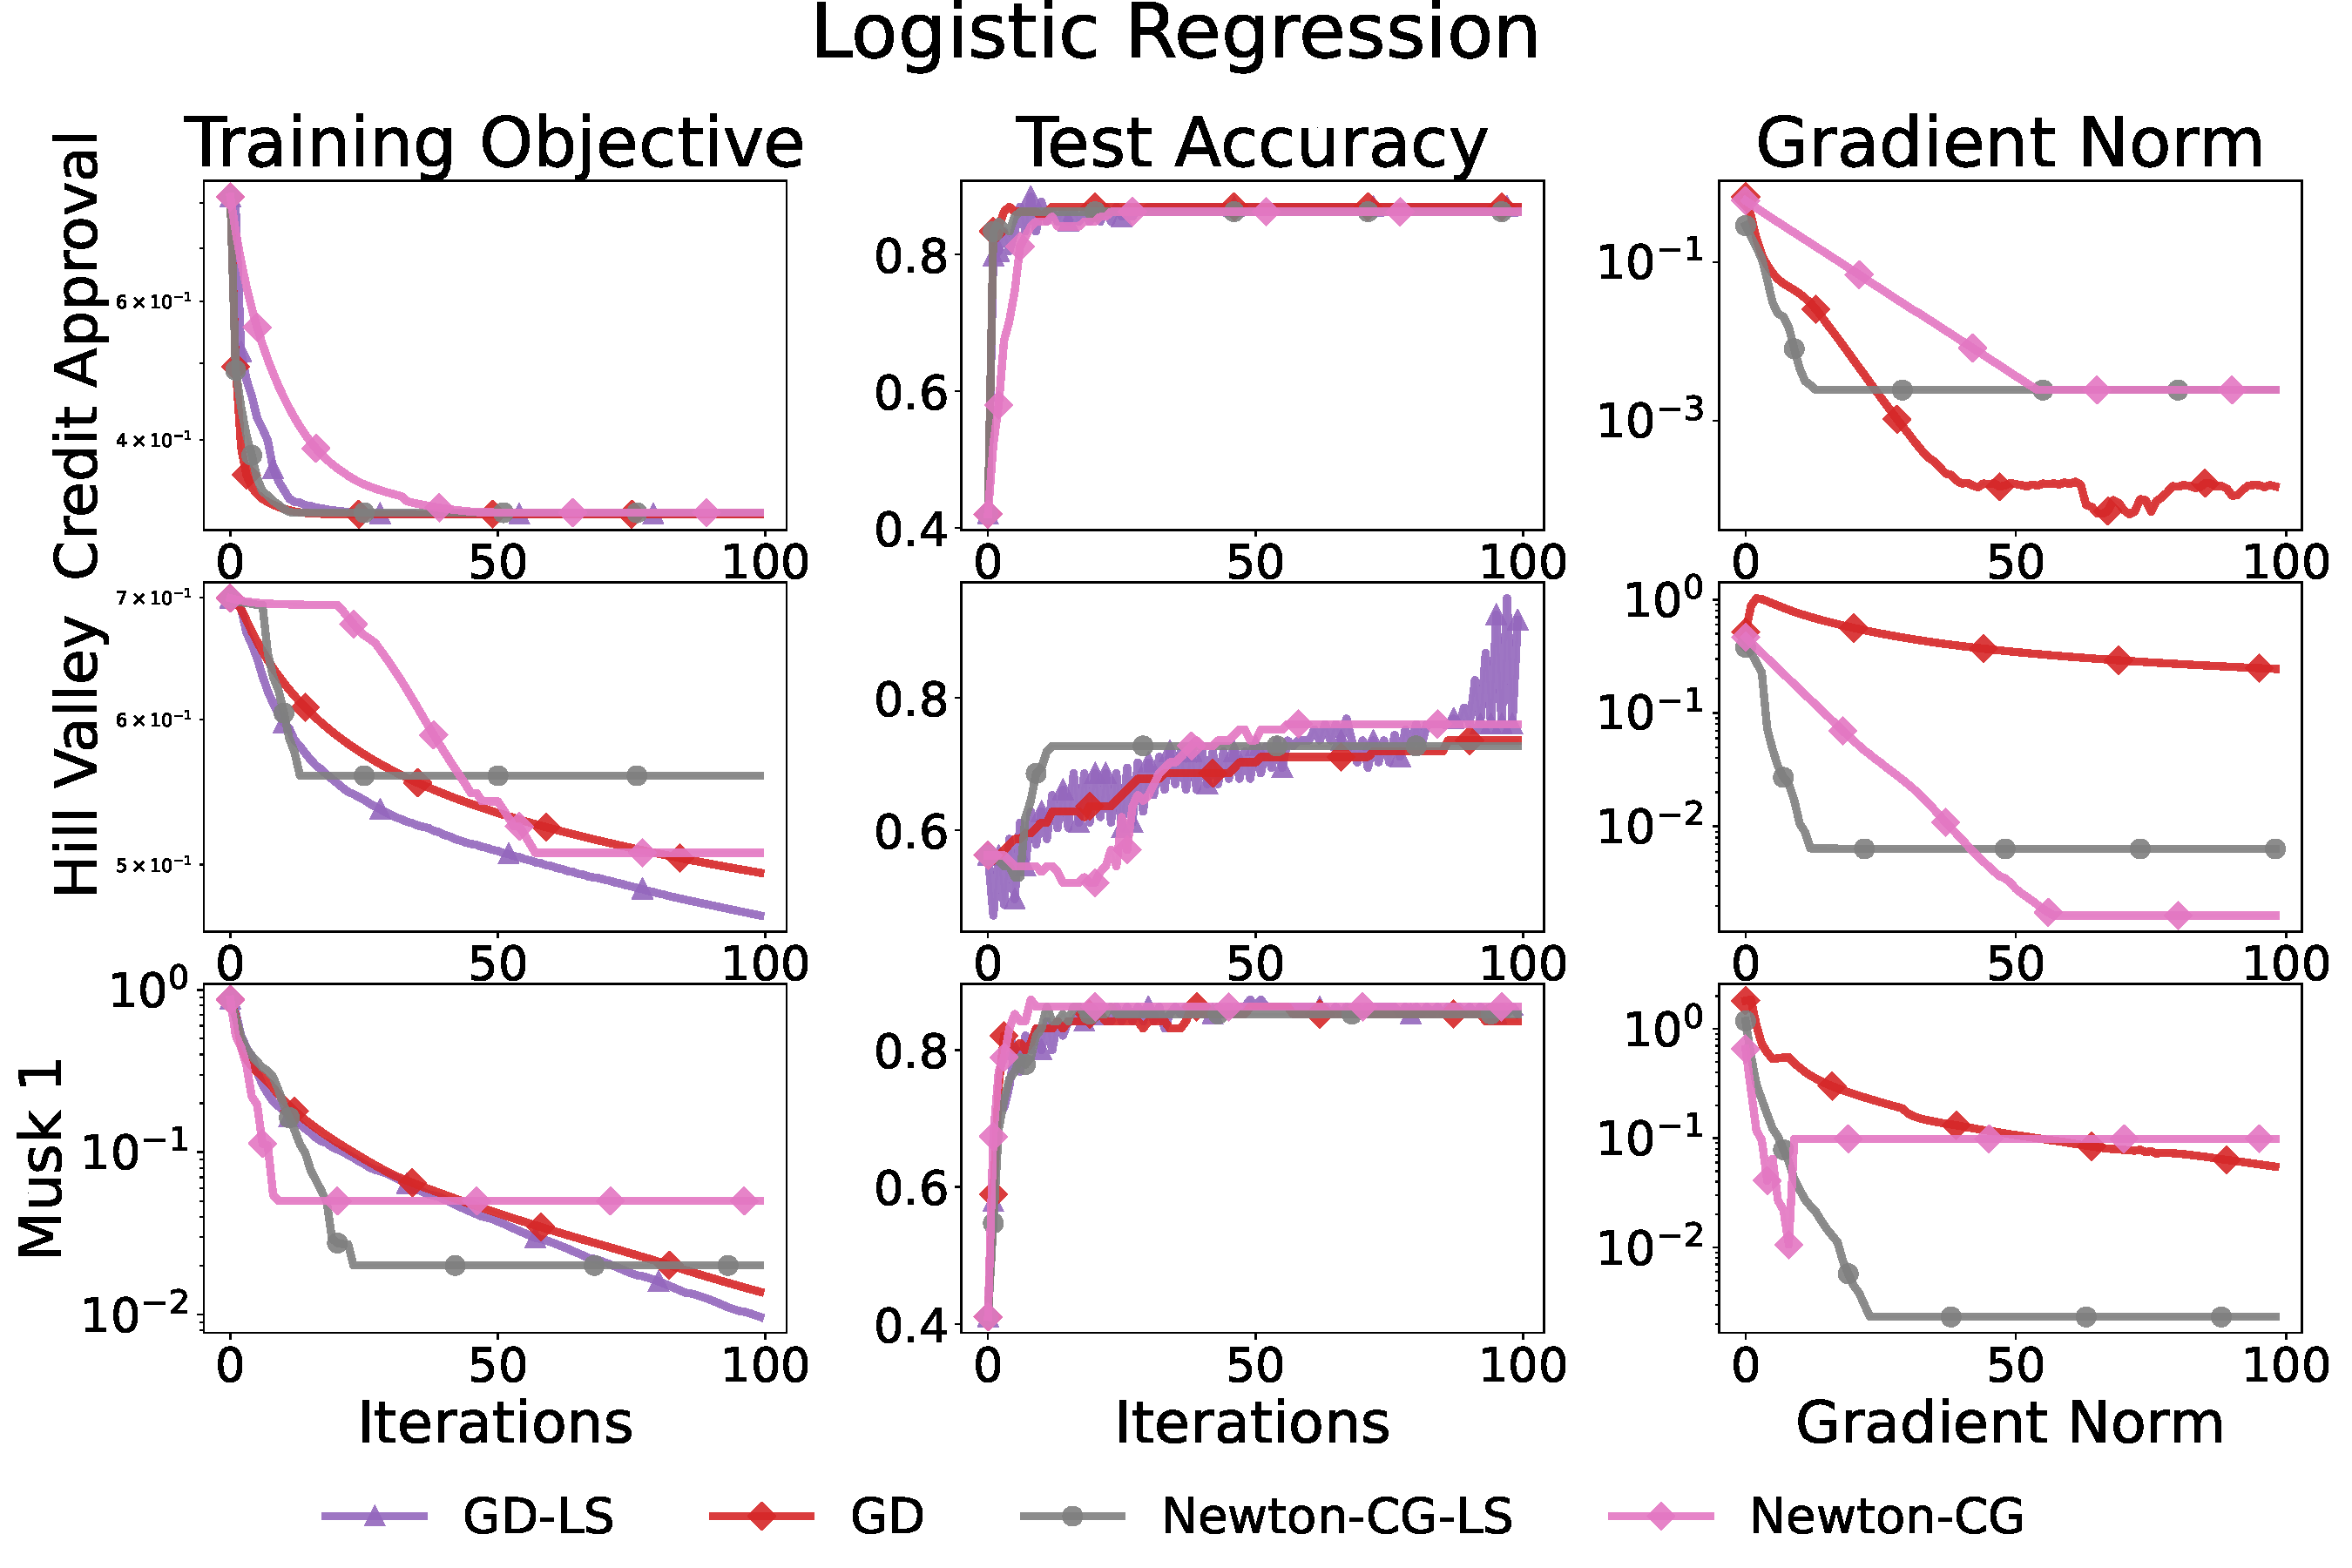
\includegraphics[width=1.0\textwidth]{assets/newton_comparison_logreg.pdf}
    \end{figure}

\end{frame}

\begin{frame}{Experiments: Convex Newton}

    But teleportation still works for \good{non-convex problems}!

    \pause

    \begin{figure}
        \centering
        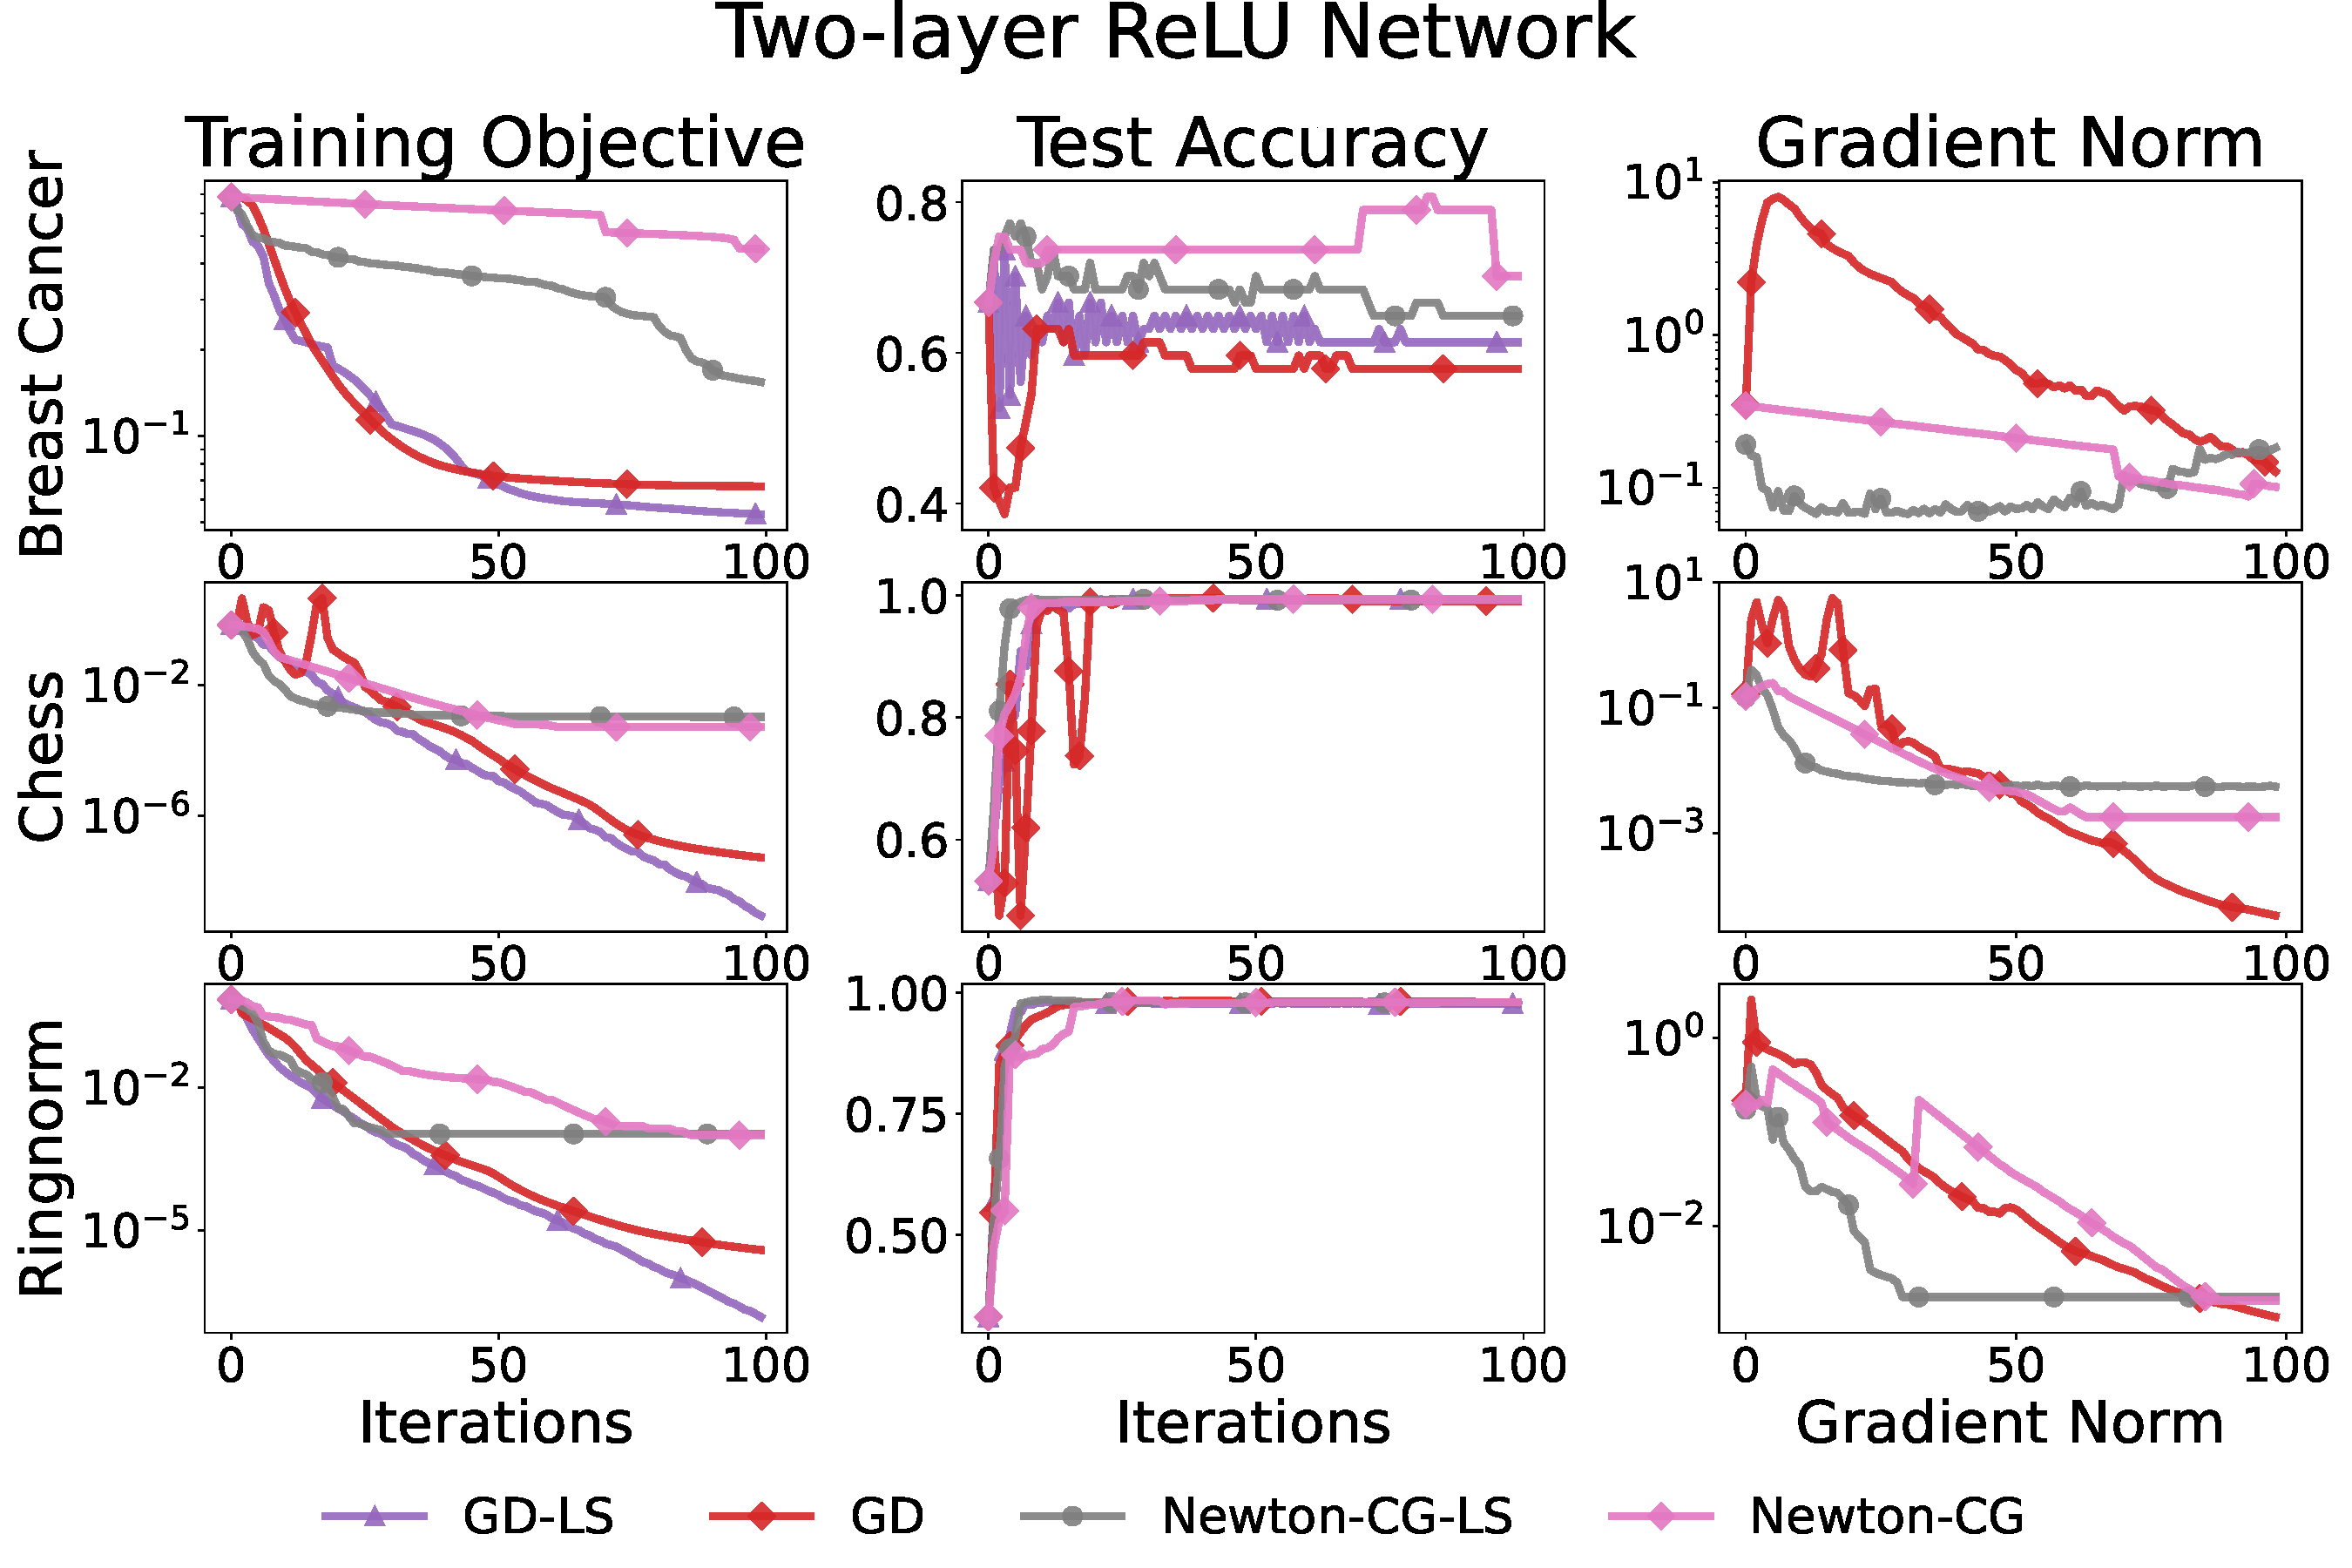
\includegraphics[width=1.0\textwidth]{assets/newton_comparison_network.pdf}
    \end{figure}

\end{frame}

\setbeamercolor{background canvas}{bg=LightCyan}
\begin{frame}{}
    \begin{center}
        \huge Questions?
    \end{center}
\end{frame}
\setbeamercolor{background canvas}{bg=white}

%% bibliography
\begin{frame}[allowframebreaks]{References}
    \printbibliography[]
\end{frame}

\end{document}
